\documentclass[twoside]{book}

% Packages required by doxygen
\usepackage{calc}
\usepackage{doxygen}
\usepackage{graphicx}
\usepackage[utf8]{inputenc}
\usepackage{makeidx}
\usepackage{multicol}
\usepackage{multirow}
\usepackage{textcomp}
\usepackage[table]{xcolor}

% Font selection
\usepackage[T1]{fontenc}
\usepackage{mathptmx}
\usepackage[scaled=.90]{helvet}
\usepackage{courier}
\usepackage{amssymb}
\usepackage{sectsty}
\renewcommand{\familydefault}{\sfdefault}
\allsectionsfont{%
  \fontseries{bc}\selectfont%
  \color{darkgray}%
}
\renewcommand{\DoxyLabelFont}{%
  \fontseries{bc}\selectfont%
  \color{darkgray}%
}

% Page & text layout
\usepackage{geometry}
\geometry{%
  a4paper,%
  top=2.5cm,%
  bottom=2.5cm,%
  left=2.5cm,%
  right=2.5cm%
}
\tolerance=750
\hfuzz=15pt
\hbadness=750
\setlength{\emergencystretch}{15pt}
\setlength{\parindent}{0cm}
\setlength{\parskip}{0.2cm}
\makeatletter
\renewcommand{\paragraph}{%
  \@startsection{paragraph}{4}{0ex}{-1.0ex}{1.0ex}{%
    \normalfont\normalsize\bfseries\SS@parafont%
  }%
}
\renewcommand{\subparagraph}{%
  \@startsection{subparagraph}{5}{0ex}{-1.0ex}{1.0ex}{%
    \normalfont\normalsize\bfseries\SS@subparafont%
  }%
}
\makeatother

% Headers & footers
\usepackage{fancyhdr}
\pagestyle{fancyplain}
\fancyhead[LE]{\fancyplain{}{\bfseries\thepage}}
\fancyhead[CE]{\fancyplain{}{}}
\fancyhead[RE]{\fancyplain{}{\bfseries\leftmark}}
\fancyhead[LO]{\fancyplain{}{\bfseries\rightmark}}
\fancyhead[CO]{\fancyplain{}{}}
\fancyhead[RO]{\fancyplain{}{\bfseries\thepage}}
\fancyfoot[LE]{\fancyplain{}{}}
\fancyfoot[CE]{\fancyplain{}{}}
\fancyfoot[RE]{\fancyplain{}{\bfseries\scriptsize Generated on Sun Mar 2 2014 23\-:05\-:17 for Hyper\-Neat by Doxygen }}
\fancyfoot[LO]{\fancyplain{}{\bfseries\scriptsize Generated on Sun Mar 2 2014 23\-:05\-:17 for Hyper\-Neat by Doxygen }}
\fancyfoot[CO]{\fancyplain{}{}}
\fancyfoot[RO]{\fancyplain{}{}}
\renewcommand{\footrulewidth}{0.4pt}
\renewcommand{\chaptermark}[1]{%
  \markboth{#1}{}%
}
\renewcommand{\sectionmark}[1]{%
  \markright{\thesection\ #1}%
}

% Indices & bibliography
\usepackage{natbib}
\usepackage[titles]{tocloft}
\setcounter{tocdepth}{3}
\setcounter{secnumdepth}{5}
\makeindex

% Hyperlinks (required, but should be loaded last)
\usepackage{ifpdf}
\ifpdf
  \usepackage[pdftex,pagebackref=true]{hyperref}
\else
  \usepackage[ps2pdf,pagebackref=true]{hyperref}
\fi
\hypersetup{%
  colorlinks=true,%
  linkcolor=blue,%
  citecolor=blue,%
  unicode%
}

% Custom commands
\newcommand{\clearemptydoublepage}{%
  \newpage{\pagestyle{empty}\cleardoublepage}%
}


%===== C O N T E N T S =====

\begin{document}

% Titlepage & ToC
\hypersetup{pageanchor=false}
\pagenumbering{roman}
\begin{titlepage}
\vspace*{7cm}
\begin{center}%
{\Large Hyper\-Neat }\\
\vspace*{1cm}
{\large Generated by Doxygen 1.8.6}\\
\vspace*{0.5cm}
{\small Sun Mar 2 2014 23:05:17}\\
\end{center}
\end{titlepage}
\clearemptydoublepage
\tableofcontents
\clearemptydoublepage
\pagenumbering{arabic}
\hypersetup{pageanchor=true}

%--- Begin generated contents ---
\chapter{Namespace Index}
\section{Namespace List}
Here is a list of all namespaces with brief descriptions\-:\begin{DoxyCompactList}
\item\contentsline{section}{\hyperlink{namespace_a_n_n___u_s_m}{A\-N\-N\-\_\-\-U\-S\-M} \\*Dedicated to artificial intelligence development in Santa María University }{\pageref{namespace_a_n_n___u_s_m}}{}
\end{DoxyCompactList}

\chapter{Class Index}
\section{Class List}
Here are the classes, structs, unions and interfaces with brief descriptions\-:\begin{DoxyCompactList}
\item\contentsline{section}{\hyperlink{class_a_n_n___u_s_m_1_1_c_p_p_n_inputs}{A\-N\-N\-\_\-\-U\-S\-M\-::\-C\-P\-P\-N\-Inputs} \\*The class \hyperlink{class_a_n_n___u_s_m_1_1_c_p_p_n_inputs}{C\-P\-P\-N\-Inputs} is used to create cppn inputs }{\pageref{class_a_n_n___u_s_m_1_1_c_p_p_n_inputs}}{}
\item\contentsline{section}{\hyperlink{class_a_n_n___u_s_m_1_1_hyper_neat}{A\-N\-N\-\_\-\-U\-S\-M\-::\-Hyper\-Neat} \\*The class \hyperlink{class_a_n_n___u_s_m_1_1_hyper_neat}{Hyper\-Neat} is used to implement a neuroevolution method called \hyperlink{class_a_n_n___u_s_m_1_1_hyper_neat}{Hyper\-Neat} }{\pageref{class_a_n_n___u_s_m_1_1_hyper_neat}}{}
\item\contentsline{section}{\hyperlink{class_a_n_n___u_s_m_1_1_spatial_connection}{A\-N\-N\-\_\-\-U\-S\-M\-::\-Spatial\-Connection} \\*The class \hyperlink{class_a_n_n___u_s_m_1_1_spatial_connection}{Spatial\-Connection} is used to create connections among overall nodes in a \hyperlink{class_a_n_n___u_s_m_1_1_hyper_neat}{Hyper\-Neat} \hyperlink{class_a_n_n___u_s_m_1_1_substrate}{Substrate} }{\pageref{class_a_n_n___u_s_m_1_1_spatial_connection}}{}
\item\contentsline{section}{\hyperlink{class_a_n_n___u_s_m_1_1_spatial_node}{A\-N\-N\-\_\-\-U\-S\-M\-::\-Spatial\-Node} \\*The class \hyperlink{class_a_n_n___u_s_m_1_1_spatial_node}{Spatial\-Node} is used to create nodes in a \hyperlink{class_a_n_n___u_s_m_1_1_hyper_neat}{Hyper\-Neat} \hyperlink{class_a_n_n___u_s_m_1_1_substrate}{Substrate} }{\pageref{class_a_n_n___u_s_m_1_1_spatial_node}}{}
\item\contentsline{section}{\hyperlink{class_a_n_n___u_s_m_1_1_substrate}{A\-N\-N\-\_\-\-U\-S\-M\-::\-Substrate} \\*The class \hyperlink{class_a_n_n___u_s_m_1_1_substrate}{Substrate} is used to create \hyperlink{class_a_n_n___u_s_m_1_1_hyper_neat}{Hyper\-Neat} \hyperlink{class_a_n_n___u_s_m_1_1_substrate}{Substrate} }{\pageref{class_a_n_n___u_s_m_1_1_substrate}}{}
\end{DoxyCompactList}

\chapter{File Index}
\section{File List}
Here is a list of all files with brief descriptions\-:\begin{DoxyCompactList}
\item\contentsline{section}{/home/oscar/\-Documents/\-Hyper\-Neat/headers/\hyperlink{_c_p_p_n_inputs_8hpp}{C\-P\-P\-N\-Inputs.\-hpp} }{\pageref{_c_p_p_n_inputs_8hpp}}{}
\item\contentsline{section}{/home/oscar/\-Documents/\-Hyper\-Neat/headers/\hyperlink{_hyper_neat_8hpp}{Hyper\-Neat.\-hpp} }{\pageref{_hyper_neat_8hpp}}{}
\item\contentsline{section}{/home/oscar/\-Documents/\-Hyper\-Neat/headers/\hyperlink{main_8hpp}{main.\-hpp} }{\pageref{main_8hpp}}{}
\item\contentsline{section}{/home/oscar/\-Documents/\-Hyper\-Neat/headers/\hyperlink{_spatial_connection_8hpp}{Spatial\-Connection.\-hpp} }{\pageref{_spatial_connection_8hpp}}{}
\item\contentsline{section}{/home/oscar/\-Documents/\-Hyper\-Neat/headers/\hyperlink{_spatial_node_8hpp}{Spatial\-Node.\-hpp} }{\pageref{_spatial_node_8hpp}}{}
\item\contentsline{section}{/home/oscar/\-Documents/\-Hyper\-Neat/headers/\hyperlink{_substrate_8hpp}{Substrate.\-hpp} }{\pageref{_substrate_8hpp}}{}
\item\contentsline{section}{/home/oscar/\-Documents/\-Hyper\-Neat/src/\hyperlink{_c_p_p_n_inputs_8cpp}{C\-P\-P\-N\-Inputs.\-cpp} }{\pageref{_c_p_p_n_inputs_8cpp}}{}
\item\contentsline{section}{/home/oscar/\-Documents/\-Hyper\-Neat/src/\hyperlink{_hyper_neat_8cpp}{Hyper\-Neat.\-cpp} }{\pageref{_hyper_neat_8cpp}}{}
\item\contentsline{section}{/home/oscar/\-Documents/\-Hyper\-Neat/src/\hyperlink{main_8cpp}{main.\-cpp} }{\pageref{main_8cpp}}{}
\item\contentsline{section}{/home/oscar/\-Documents/\-Hyper\-Neat/src/\hyperlink{_spatial_connection_8cpp}{Spatial\-Connection.\-cpp} }{\pageref{_spatial_connection_8cpp}}{}
\item\contentsline{section}{/home/oscar/\-Documents/\-Hyper\-Neat/src/\hyperlink{_spatial_node_8cpp}{Spatial\-Node.\-cpp} }{\pageref{_spatial_node_8cpp}}{}
\item\contentsline{section}{/home/oscar/\-Documents/\-Hyper\-Neat/src/\hyperlink{_substrate_8cpp}{Substrate.\-cpp} }{\pageref{_substrate_8cpp}}{}
\end{DoxyCompactList}

\chapter{Namespace Documentation}
\hypertarget{namespace_a_n_n___u_s_m}{\section{A\-N\-N\-\_\-\-U\-S\-M Namespace Reference}
\label{namespace_a_n_n___u_s_m}\index{A\-N\-N\-\_\-\-U\-S\-M@{A\-N\-N\-\_\-\-U\-S\-M}}
}


Dedicated to artificial intelligence development in Santa María University.  


\subsection*{Classes}
\begin{DoxyCompactItemize}
\item 
class \hyperlink{class_a_n_n___u_s_m_1_1_c_p_p_n_inputs}{C\-P\-P\-N\-Inputs}
\begin{DoxyCompactList}\small\item\em The class \hyperlink{class_a_n_n___u_s_m_1_1_c_p_p_n_inputs}{C\-P\-P\-N\-Inputs} is used to create cppn inputs. \end{DoxyCompactList}\item 
class \hyperlink{class_a_n_n___u_s_m_1_1_hyper_neat}{Hyper\-Neat}
\begin{DoxyCompactList}\small\item\em The class \hyperlink{class_a_n_n___u_s_m_1_1_hyper_neat}{Hyper\-Neat} is used to implement a neuroevolution method called \hyperlink{class_a_n_n___u_s_m_1_1_hyper_neat}{Hyper\-Neat}. \end{DoxyCompactList}\item 
class \hyperlink{class_a_n_n___u_s_m_1_1_spatial_connection}{Spatial\-Connection}
\begin{DoxyCompactList}\small\item\em The class \hyperlink{class_a_n_n___u_s_m_1_1_spatial_connection}{Spatial\-Connection} is used to create connections among overall nodes in a \hyperlink{class_a_n_n___u_s_m_1_1_hyper_neat}{Hyper\-Neat} \hyperlink{class_a_n_n___u_s_m_1_1_substrate}{Substrate}. \end{DoxyCompactList}\item 
class \hyperlink{class_a_n_n___u_s_m_1_1_spatial_node}{Spatial\-Node}
\begin{DoxyCompactList}\small\item\em The class \hyperlink{class_a_n_n___u_s_m_1_1_spatial_node}{Spatial\-Node} is used to create nodes in a \hyperlink{class_a_n_n___u_s_m_1_1_hyper_neat}{Hyper\-Neat} \hyperlink{class_a_n_n___u_s_m_1_1_substrate}{Substrate}. \end{DoxyCompactList}\item 
class \hyperlink{class_a_n_n___u_s_m_1_1_substrate}{Substrate}
\begin{DoxyCompactList}\small\item\em The class \hyperlink{class_a_n_n___u_s_m_1_1_substrate}{Substrate} is used to create \hyperlink{class_a_n_n___u_s_m_1_1_hyper_neat}{Hyper\-Neat} \hyperlink{class_a_n_n___u_s_m_1_1_substrate}{Substrate}. \end{DoxyCompactList}\end{DoxyCompactItemize}


\subsection{Detailed Description}
Dedicated to artificial intelligence development in Santa María University. 
\chapter{Class Documentation}
\hypertarget{class_a_n_n___u_s_m_1_1_c_p_p_n_inputs}{\section{A\-N\-N\-\_\-\-U\-S\-M\-:\-:C\-P\-P\-N\-Inputs Class Reference}
\label{class_a_n_n___u_s_m_1_1_c_p_p_n_inputs}\index{A\-N\-N\-\_\-\-U\-S\-M\-::\-C\-P\-P\-N\-Inputs@{A\-N\-N\-\_\-\-U\-S\-M\-::\-C\-P\-P\-N\-Inputs}}
}


The class \hyperlink{class_a_n_n___u_s_m_1_1_c_p_p_n_inputs}{C\-P\-P\-N\-Inputs} is used to create cppn inputs.  




{\ttfamily \#include $<$C\-P\-P\-N\-Inputs.\-hpp$>$}

\subsection*{Public Member Functions}
\begin{DoxyCompactItemize}
\item 
\hyperlink{class_a_n_n___u_s_m_1_1_c_p_p_n_inputs_a8e11fc60cf97088554222a49a9e2138d}{C\-P\-P\-N\-Inputs} (char $\ast$type, double bias)
\begin{DoxyCompactList}\small\item\em Constructor. \end{DoxyCompactList}\item 
\hyperlink{class_a_n_n___u_s_m_1_1_c_p_p_n_inputs_a4cf182897edc0aab6396309fb805d17d}{$\sim$\-C\-P\-P\-N\-Inputs} ()
\begin{DoxyCompactList}\small\item\em Destructor. \end{DoxyCompactList}\item 
double \hyperlink{class_a_n_n___u_s_m_1_1_c_p_p_n_inputs_a2d83e6f6066f241024a435f23aaf6519}{Eval} (vector$<$ double $>$ point)
\begin{DoxyCompactList}\small\item\em Eval function. Eval the function corresponding to type name. \end{DoxyCompactList}\item 
char $\ast$ \hyperlink{class_a_n_n___u_s_m_1_1_c_p_p_n_inputs_af3b8e063ed149d720edcd4baab27e948}{Get\-Type} ()
\begin{DoxyCompactList}\small\item\em Get cppn input type name. \end{DoxyCompactList}\end{DoxyCompactItemize}


\subsection{Detailed Description}
The class \hyperlink{class_a_n_n___u_s_m_1_1_c_p_p_n_inputs}{C\-P\-P\-N\-Inputs} is used to create cppn inputs. 

Definition at line 18 of file C\-P\-P\-N\-Inputs.\-hpp.



\subsection{Constructor \& Destructor Documentation}
\hypertarget{class_a_n_n___u_s_m_1_1_c_p_p_n_inputs_a8e11fc60cf97088554222a49a9e2138d}{\index{A\-N\-N\-\_\-\-U\-S\-M\-::\-C\-P\-P\-N\-Inputs@{A\-N\-N\-\_\-\-U\-S\-M\-::\-C\-P\-P\-N\-Inputs}!C\-P\-P\-N\-Inputs@{C\-P\-P\-N\-Inputs}}
\index{C\-P\-P\-N\-Inputs@{C\-P\-P\-N\-Inputs}!ANN_USM::CPPNInputs@{A\-N\-N\-\_\-\-U\-S\-M\-::\-C\-P\-P\-N\-Inputs}}
\subsubsection[{C\-P\-P\-N\-Inputs}]{\setlength{\rightskip}{0pt plus 5cm}C\-P\-P\-N\-Inputs\-::\-C\-P\-P\-N\-Inputs (
\begin{DoxyParamCaption}
\item[{char $\ast$}]{type, }
\item[{double}]{bias}
\end{DoxyParamCaption}
)}}\label{class_a_n_n___u_s_m_1_1_c_p_p_n_inputs_a8e11fc60cf97088554222a49a9e2138d}


Constructor. 


\begin{DoxyParams}{Parameters}
{\em type} & Char array with the input type name. \\
\hline
{\em bias} & If the input corresponds to bias input, this variable store a bias input value. \\
\hline
\end{DoxyParams}


Definition at line 7 of file C\-P\-P\-N\-Inputs.\-cpp.

\hypertarget{class_a_n_n___u_s_m_1_1_c_p_p_n_inputs_a4cf182897edc0aab6396309fb805d17d}{\index{A\-N\-N\-\_\-\-U\-S\-M\-::\-C\-P\-P\-N\-Inputs@{A\-N\-N\-\_\-\-U\-S\-M\-::\-C\-P\-P\-N\-Inputs}!$\sim$\-C\-P\-P\-N\-Inputs@{$\sim$\-C\-P\-P\-N\-Inputs}}
\index{$\sim$\-C\-P\-P\-N\-Inputs@{$\sim$\-C\-P\-P\-N\-Inputs}!ANN_USM::CPPNInputs@{A\-N\-N\-\_\-\-U\-S\-M\-::\-C\-P\-P\-N\-Inputs}}
\subsubsection[{$\sim$\-C\-P\-P\-N\-Inputs}]{\setlength{\rightskip}{0pt plus 5cm}C\-P\-P\-N\-Inputs\-::$\sim$\-C\-P\-P\-N\-Inputs (
\begin{DoxyParamCaption}
{}
\end{DoxyParamCaption}
)}}\label{class_a_n_n___u_s_m_1_1_c_p_p_n_inputs_a4cf182897edc0aab6396309fb805d17d}


Destructor. 



Definition at line 27 of file C\-P\-P\-N\-Inputs.\-cpp.



\subsection{Member Function Documentation}
\hypertarget{class_a_n_n___u_s_m_1_1_c_p_p_n_inputs_a2d83e6f6066f241024a435f23aaf6519}{\index{A\-N\-N\-\_\-\-U\-S\-M\-::\-C\-P\-P\-N\-Inputs@{A\-N\-N\-\_\-\-U\-S\-M\-::\-C\-P\-P\-N\-Inputs}!Eval@{Eval}}
\index{Eval@{Eval}!ANN_USM::CPPNInputs@{A\-N\-N\-\_\-\-U\-S\-M\-::\-C\-P\-P\-N\-Inputs}}
\subsubsection[{Eval}]{\setlength{\rightskip}{0pt plus 5cm}double C\-P\-P\-N\-Inputs\-::\-Eval (
\begin{DoxyParamCaption}
\item[{vector$<$ double $>$}]{point}
\end{DoxyParamCaption}
)}}\label{class_a_n_n___u_s_m_1_1_c_p_p_n_inputs_a2d83e6f6066f241024a435f23aaf6519}


Eval function. Eval the function corresponding to type name. 


\begin{DoxyParams}{Parameters}
{\em point} & Vector of coordenate of each node, source and target. \\
\hline
\end{DoxyParams}
\begin{DoxyReturn}{Returns}
Returned value of function corresponding to type name. 
\end{DoxyReturn}


Definition at line 29 of file C\-P\-P\-N\-Inputs.\-cpp.

\hypertarget{class_a_n_n___u_s_m_1_1_c_p_p_n_inputs_af3b8e063ed149d720edcd4baab27e948}{\index{A\-N\-N\-\_\-\-U\-S\-M\-::\-C\-P\-P\-N\-Inputs@{A\-N\-N\-\_\-\-U\-S\-M\-::\-C\-P\-P\-N\-Inputs}!Get\-Type@{Get\-Type}}
\index{Get\-Type@{Get\-Type}!ANN_USM::CPPNInputs@{A\-N\-N\-\_\-\-U\-S\-M\-::\-C\-P\-P\-N\-Inputs}}
\subsubsection[{Get\-Type}]{\setlength{\rightskip}{0pt plus 5cm}char $\ast$ C\-P\-P\-N\-Inputs\-::\-Get\-Type (
\begin{DoxyParamCaption}
{}
\end{DoxyParamCaption}
)}}\label{class_a_n_n___u_s_m_1_1_c_p_p_n_inputs_af3b8e063ed149d720edcd4baab27e948}


Get cppn input type name. 

\begin{DoxyReturn}{Returns}
Char array with type name. 
\end{DoxyReturn}


Definition at line 53 of file C\-P\-P\-N\-Inputs.\-cpp.



The documentation for this class was generated from the following files\-:\begin{DoxyCompactItemize}
\item 
/home/oscar/\-Documents/\-Hyper\-Neat/headers/\hyperlink{_c_p_p_n_inputs_8hpp}{C\-P\-P\-N\-Inputs.\-hpp}\item 
/home/oscar/\-Documents/\-Hyper\-Neat/src/\hyperlink{_c_p_p_n_inputs_8cpp}{C\-P\-P\-N\-Inputs.\-cpp}\end{DoxyCompactItemize}

\hypertarget{class_a_n_n___u_s_m_1_1_hyper_neat}{\section{A\-N\-N\-\_\-\-U\-S\-M\-:\-:Hyper\-Neat Class Reference}
\label{class_a_n_n___u_s_m_1_1_hyper_neat}\index{A\-N\-N\-\_\-\-U\-S\-M\-::\-Hyper\-Neat@{A\-N\-N\-\_\-\-U\-S\-M\-::\-Hyper\-Neat}}
}


The class \hyperlink{class_a_n_n___u_s_m_1_1_hyper_neat}{Hyper\-Neat} is used to implement a neuroevolution method called \hyperlink{class_a_n_n___u_s_m_1_1_hyper_neat}{Hyper\-Neat}.  




{\ttfamily \#include $<$Hyper\-Neat.\-hpp$>$}

\subsection*{Public Member Functions}
\begin{DoxyCompactItemize}
\item 
\hyperlink{class_a_n_n___u_s_m_1_1_hyper_neat_afa5ee92982d0a780e485341722a00286}{Hyper\-Neat} (vector$<$ double $\ast$ $>$ inputs, vector$<$ double $\ast$ $>$ outputs, string hyperneat\-\_\-info)
\begin{DoxyCompactList}\small\item\em Constructor with parameters. \end{DoxyCompactList}\item 
\hyperlink{class_a_n_n___u_s_m_1_1_hyper_neat_a1cd44e92cbfd6902977aad68ab7585ed}{$\sim$\-Hyper\-Neat} ()
\begin{DoxyCompactList}\small\item\em Destructor. \end{DoxyCompactList}\item 
void \hyperlink{class_a_n_n___u_s_m_1_1_hyper_neat_a67803bb6c5dc5986d9c44877d92587af}{H\-Json\-Deserialize} (string hyperneat\-\_\-info)
\begin{DoxyCompactList}\small\item\em Extract all \hyperlink{class_a_n_n___u_s_m_1_1_hyper_neat}{Hyper\-Neat} information of json string. \end{DoxyCompactList}\item 
void \hyperlink{class_a_n_n___u_s_m_1_1_hyper_neat_a0eb24949bc741c24f12bd812d519de8c}{Create\-Substrate\-Connections} ()
\begin{DoxyCompactList}\small\item\em Create all substrate connections according to cppn-\/neat result. \end{DoxyCompactList}\item 
void \hyperlink{class_a_n_n___u_s_m_1_1_hyper_neat_a593bcca0140041a340814b91d29a4a13}{Evaluate\-Substrate\-Connections} ()
\begin{DoxyCompactList}\small\item\em Allows to obtain the final \hyperlink{class_a_n_n___u_s_m_1_1_hyper_neat}{Hyper\-Neat} outputs. \end{DoxyCompactList}\item 
void \hyperlink{class_a_n_n___u_s_m_1_1_hyper_neat_aa2db8cfc0f567d330c07fbc209ad1bf2}{Evaluate\-Connections} (int sheet\-\_\-num)
\begin{DoxyCompactList}\small\item\em Evaluate all connections after specific sheet. \end{DoxyCompactList}\end{DoxyCompactItemize}


\subsection{Detailed Description}
The class \hyperlink{class_a_n_n___u_s_m_1_1_hyper_neat}{Hyper\-Neat} is used to implement a neuroevolution method called \hyperlink{class_a_n_n___u_s_m_1_1_hyper_neat}{Hyper\-Neat}. 

Definition at line 22 of file Hyper\-Neat.\-hpp.



\subsection{Constructor \& Destructor Documentation}
\hypertarget{class_a_n_n___u_s_m_1_1_hyper_neat_afa5ee92982d0a780e485341722a00286}{\index{A\-N\-N\-\_\-\-U\-S\-M\-::\-Hyper\-Neat@{A\-N\-N\-\_\-\-U\-S\-M\-::\-Hyper\-Neat}!Hyper\-Neat@{Hyper\-Neat}}
\index{Hyper\-Neat@{Hyper\-Neat}!ANN_USM::HyperNeat@{A\-N\-N\-\_\-\-U\-S\-M\-::\-Hyper\-Neat}}
\subsubsection[{Hyper\-Neat}]{\setlength{\rightskip}{0pt plus 5cm}Hyper\-Neat\-::\-Hyper\-Neat (
\begin{DoxyParamCaption}
\item[{vector$<$ double $\ast$ $>$}]{inputs, }
\item[{vector$<$ double $\ast$ $>$}]{outputs, }
\item[{string}]{hyperneat\-\_\-info}
\end{DoxyParamCaption}
)}}\label{class_a_n_n___u_s_m_1_1_hyper_neat_afa5ee92982d0a780e485341722a00286}


Constructor with parameters. 


\begin{DoxyParams}{Parameters}
{\em inputs} & Input vector \\
\hline
{\em outputs} & Output vector \\
\hline
{\em hyperneat\-\_\-info} & Json string \\
\hline
\end{DoxyParams}


Definition at line 10 of file Hyper\-Neat.\-cpp.



Here is the call graph for this function\-:\nopagebreak
\begin{figure}[H]
\begin{center}
\leavevmode
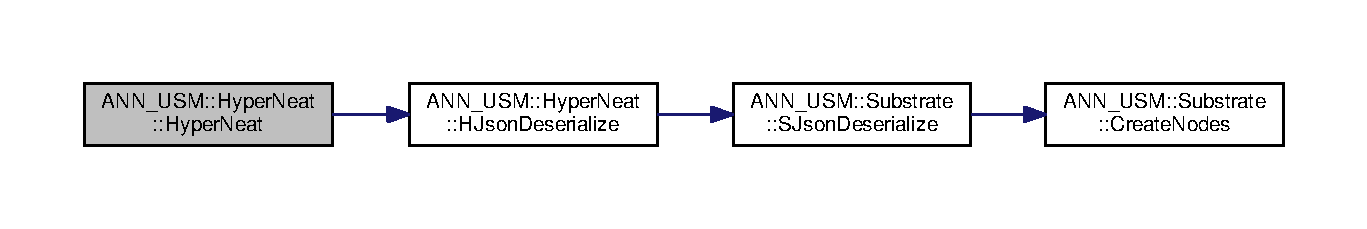
\includegraphics[width=350pt]{class_a_n_n___u_s_m_1_1_hyper_neat_afa5ee92982d0a780e485341722a00286_cgraph}
\end{center}
\end{figure}


\hypertarget{class_a_n_n___u_s_m_1_1_hyper_neat_a1cd44e92cbfd6902977aad68ab7585ed}{\index{A\-N\-N\-\_\-\-U\-S\-M\-::\-Hyper\-Neat@{A\-N\-N\-\_\-\-U\-S\-M\-::\-Hyper\-Neat}!$\sim$\-Hyper\-Neat@{$\sim$\-Hyper\-Neat}}
\index{$\sim$\-Hyper\-Neat@{$\sim$\-Hyper\-Neat}!ANN_USM::HyperNeat@{A\-N\-N\-\_\-\-U\-S\-M\-::\-Hyper\-Neat}}
\subsubsection[{$\sim$\-Hyper\-Neat}]{\setlength{\rightskip}{0pt plus 5cm}Hyper\-Neat\-::$\sim$\-Hyper\-Neat (
\begin{DoxyParamCaption}
{}
\end{DoxyParamCaption}
)}}\label{class_a_n_n___u_s_m_1_1_hyper_neat_a1cd44e92cbfd6902977aad68ab7585ed}


Destructor. 



Definition at line 17 of file Hyper\-Neat.\-cpp.



\subsection{Member Function Documentation}
\hypertarget{class_a_n_n___u_s_m_1_1_hyper_neat_a0eb24949bc741c24f12bd812d519de8c}{\index{A\-N\-N\-\_\-\-U\-S\-M\-::\-Hyper\-Neat@{A\-N\-N\-\_\-\-U\-S\-M\-::\-Hyper\-Neat}!Create\-Substrate\-Connections@{Create\-Substrate\-Connections}}
\index{Create\-Substrate\-Connections@{Create\-Substrate\-Connections}!ANN_USM::HyperNeat@{A\-N\-N\-\_\-\-U\-S\-M\-::\-Hyper\-Neat}}
\subsubsection[{Create\-Substrate\-Connections}]{\setlength{\rightskip}{0pt plus 5cm}void Hyper\-Neat\-::\-Create\-Substrate\-Connections (
\begin{DoxyParamCaption}
{}
\end{DoxyParamCaption}
)}}\label{class_a_n_n___u_s_m_1_1_hyper_neat_a0eb24949bc741c24f12bd812d519de8c}


Create all substrate connections according to cppn-\/neat result. 



Definition at line 61 of file Hyper\-Neat.\-cpp.



Here is the call graph for this function\-:\nopagebreak
\begin{figure}[H]
\begin{center}
\leavevmode
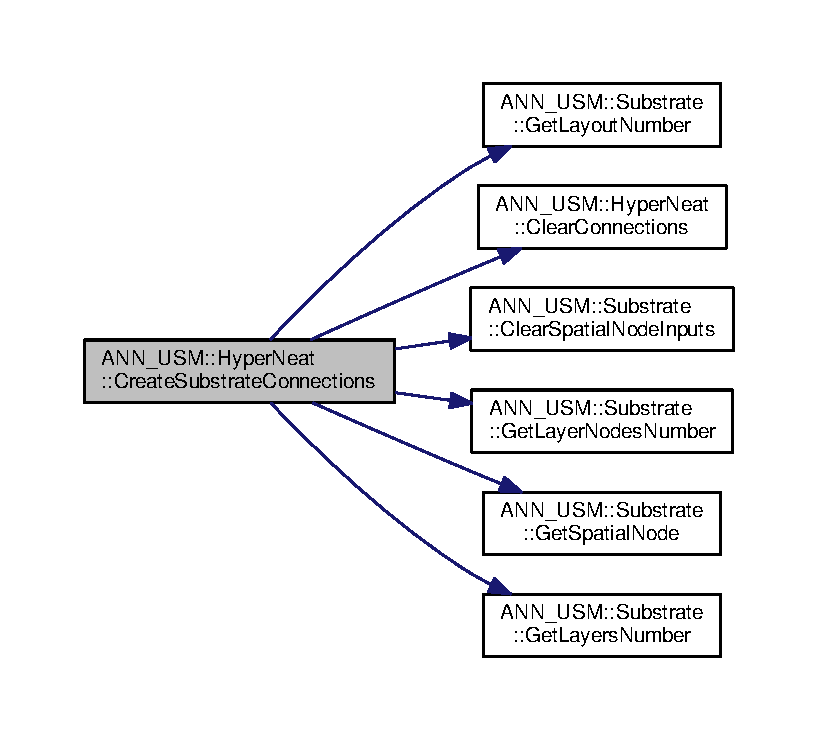
\includegraphics[width=350pt]{class_a_n_n___u_s_m_1_1_hyper_neat_a0eb24949bc741c24f12bd812d519de8c_cgraph}
\end{center}
\end{figure}




Here is the caller graph for this function\-:\nopagebreak
\begin{figure}[H]
\begin{center}
\leavevmode
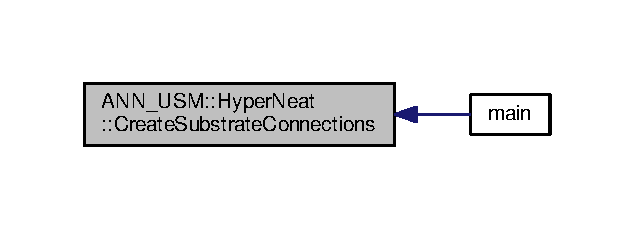
\includegraphics[width=304pt]{class_a_n_n___u_s_m_1_1_hyper_neat_a0eb24949bc741c24f12bd812d519de8c_icgraph}
\end{center}
\end{figure}


\hypertarget{class_a_n_n___u_s_m_1_1_hyper_neat_aa2db8cfc0f567d330c07fbc209ad1bf2}{\index{A\-N\-N\-\_\-\-U\-S\-M\-::\-Hyper\-Neat@{A\-N\-N\-\_\-\-U\-S\-M\-::\-Hyper\-Neat}!Evaluate\-Connections@{Evaluate\-Connections}}
\index{Evaluate\-Connections@{Evaluate\-Connections}!ANN_USM::HyperNeat@{A\-N\-N\-\_\-\-U\-S\-M\-::\-Hyper\-Neat}}
\subsubsection[{Evaluate\-Connections}]{\setlength{\rightskip}{0pt plus 5cm}void Hyper\-Neat\-::\-Evaluate\-Connections (
\begin{DoxyParamCaption}
\item[{int}]{sheet\-\_\-num}
\end{DoxyParamCaption}
)}}\label{class_a_n_n___u_s_m_1_1_hyper_neat_aa2db8cfc0f567d330c07fbc209ad1bf2}


Evaluate all connections after specific sheet. 


\begin{DoxyParams}{Parameters}
{\em sheet\-\_\-num} & Sheet number \\
\hline
\end{DoxyParams}


Definition at line 141 of file Hyper\-Neat.\-cpp.



Here is the caller graph for this function\-:\nopagebreak
\begin{figure}[H]
\begin{center}
\leavevmode
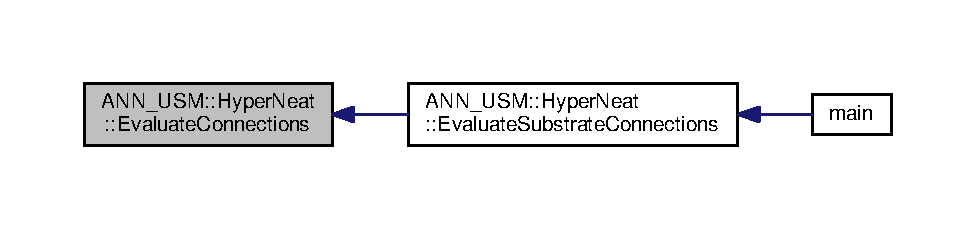
\includegraphics[width=350pt]{class_a_n_n___u_s_m_1_1_hyper_neat_aa2db8cfc0f567d330c07fbc209ad1bf2_icgraph}
\end{center}
\end{figure}


\hypertarget{class_a_n_n___u_s_m_1_1_hyper_neat_a593bcca0140041a340814b91d29a4a13}{\index{A\-N\-N\-\_\-\-U\-S\-M\-::\-Hyper\-Neat@{A\-N\-N\-\_\-\-U\-S\-M\-::\-Hyper\-Neat}!Evaluate\-Substrate\-Connections@{Evaluate\-Substrate\-Connections}}
\index{Evaluate\-Substrate\-Connections@{Evaluate\-Substrate\-Connections}!ANN_USM::HyperNeat@{A\-N\-N\-\_\-\-U\-S\-M\-::\-Hyper\-Neat}}
\subsubsection[{Evaluate\-Substrate\-Connections}]{\setlength{\rightskip}{0pt plus 5cm}void Hyper\-Neat\-::\-Evaluate\-Substrate\-Connections (
\begin{DoxyParamCaption}
{}
\end{DoxyParamCaption}
)}}\label{class_a_n_n___u_s_m_1_1_hyper_neat_a593bcca0140041a340814b91d29a4a13}


Allows to obtain the final \hyperlink{class_a_n_n___u_s_m_1_1_hyper_neat}{Hyper\-Neat} outputs. 



Definition at line 117 of file Hyper\-Neat.\-cpp.



Here is the call graph for this function\-:\nopagebreak
\begin{figure}[H]
\begin{center}
\leavevmode
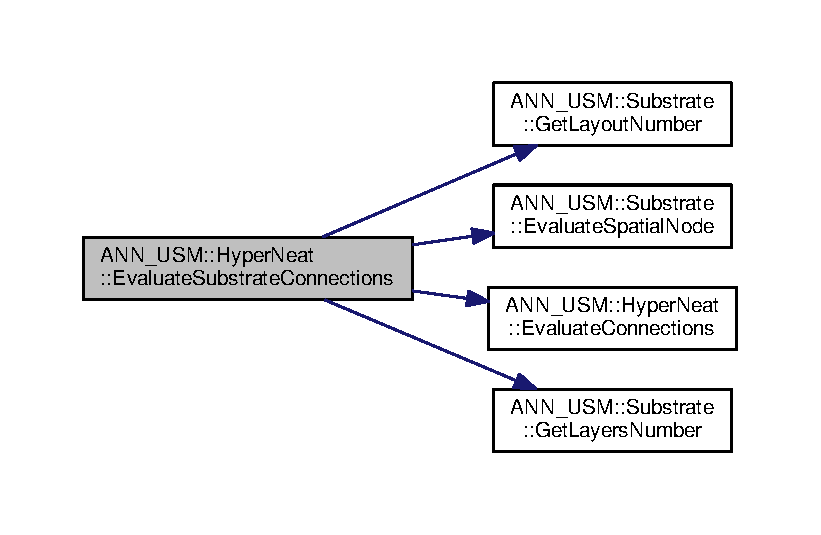
\includegraphics[width=350pt]{class_a_n_n___u_s_m_1_1_hyper_neat_a593bcca0140041a340814b91d29a4a13_cgraph}
\end{center}
\end{figure}




Here is the caller graph for this function\-:\nopagebreak
\begin{figure}[H]
\begin{center}
\leavevmode
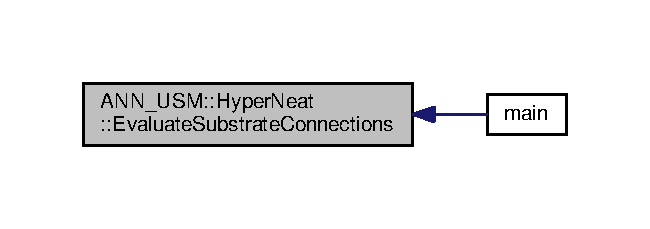
\includegraphics[width=312pt]{class_a_n_n___u_s_m_1_1_hyper_neat_a593bcca0140041a340814b91d29a4a13_icgraph}
\end{center}
\end{figure}


\hypertarget{class_a_n_n___u_s_m_1_1_hyper_neat_a67803bb6c5dc5986d9c44877d92587af}{\index{A\-N\-N\-\_\-\-U\-S\-M\-::\-Hyper\-Neat@{A\-N\-N\-\_\-\-U\-S\-M\-::\-Hyper\-Neat}!H\-Json\-Deserialize@{H\-Json\-Deserialize}}
\index{H\-Json\-Deserialize@{H\-Json\-Deserialize}!ANN_USM::HyperNeat@{A\-N\-N\-\_\-\-U\-S\-M\-::\-Hyper\-Neat}}
\subsubsection[{H\-Json\-Deserialize}]{\setlength{\rightskip}{0pt plus 5cm}void Hyper\-Neat\-::\-H\-Json\-Deserialize (
\begin{DoxyParamCaption}
\item[{string}]{hyperneat\-\_\-info}
\end{DoxyParamCaption}
)}}\label{class_a_n_n___u_s_m_1_1_hyper_neat_a67803bb6c5dc5986d9c44877d92587af}


Extract all \hyperlink{class_a_n_n___u_s_m_1_1_hyper_neat}{Hyper\-Neat} information of json string. 


\begin{DoxyParams}{Parameters}
{\em hyperneat\-\_\-info} & json string \\
\hline
\end{DoxyParams}


Definition at line 23 of file Hyper\-Neat.\-cpp.



Here is the call graph for this function\-:\nopagebreak
\begin{figure}[H]
\begin{center}
\leavevmode
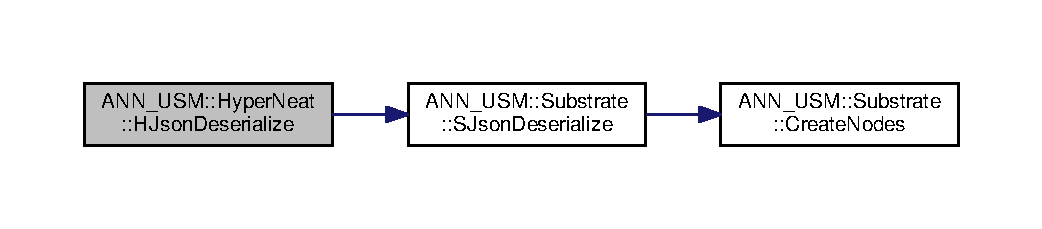
\includegraphics[width=350pt]{class_a_n_n___u_s_m_1_1_hyper_neat_a67803bb6c5dc5986d9c44877d92587af_cgraph}
\end{center}
\end{figure}




Here is the caller graph for this function\-:\nopagebreak
\begin{figure}[H]
\begin{center}
\leavevmode
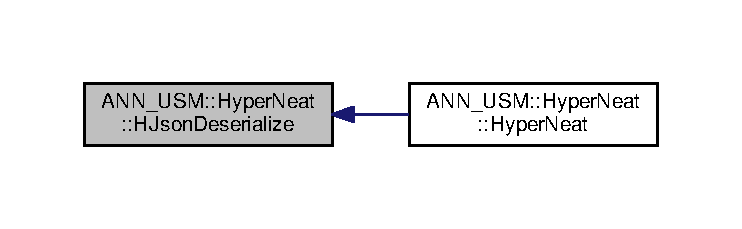
\includegraphics[width=350pt]{class_a_n_n___u_s_m_1_1_hyper_neat_a67803bb6c5dc5986d9c44877d92587af_icgraph}
\end{center}
\end{figure}




The documentation for this class was generated from the following files\-:\begin{DoxyCompactItemize}
\item 
/home/oscar/\-Documents/\-Hyper\-Neat/headers/\hyperlink{_hyper_neat_8hpp}{Hyper\-Neat.\-hpp}\item 
/home/oscar/\-Documents/\-Hyper\-Neat/src/\hyperlink{_hyper_neat_8cpp}{Hyper\-Neat.\-cpp}\end{DoxyCompactItemize}

\hypertarget{class_a_n_n___u_s_m_1_1_spatial_connection}{\section{A\-N\-N\-\_\-\-U\-S\-M\-:\-:Spatial\-Connection Class Reference}
\label{class_a_n_n___u_s_m_1_1_spatial_connection}\index{A\-N\-N\-\_\-\-U\-S\-M\-::\-Spatial\-Connection@{A\-N\-N\-\_\-\-U\-S\-M\-::\-Spatial\-Connection}}
}


The class \hyperlink{class_a_n_n___u_s_m_1_1_spatial_connection}{Spatial\-Connection} is used to create connections among overall nodes in a \hyperlink{class_a_n_n___u_s_m_1_1_hyper_neat}{Hyper\-Neat} \hyperlink{class_a_n_n___u_s_m_1_1_substrate}{Substrate}.  




{\ttfamily \#include $<$Spatial\-Connection.\-hpp$>$}

\subsection*{Public Member Functions}
\begin{DoxyCompactItemize}
\item 
\hyperlink{class_a_n_n___u_s_m_1_1_spatial_connection_a2043e25434c9f6de7d49f878499b40c9}{Spatial\-Connection} (\hyperlink{class_a_n_n___u_s_m_1_1_spatial_node}{Spatial\-Node} $\ast$input\-\_\-node, \hyperlink{class_a_n_n___u_s_m_1_1_spatial_node}{Spatial\-Node} $\ast$output\-\_\-node, double weight)
\begin{DoxyCompactList}\small\item\em Constructor. \end{DoxyCompactList}\item 
\hyperlink{class_a_n_n___u_s_m_1_1_spatial_connection_a9965054cf2e32331a537ed19f79f9c1b}{$\sim$\-Spatial\-Connection} ()
\begin{DoxyCompactList}\small\item\em Destructor. \end{DoxyCompactList}\item 
void \hyperlink{class_a_n_n___u_s_m_1_1_spatial_connection_a6966fadad1b8fc5c538756bd960f5330}{Evaluate} ()
\begin{DoxyCompactList}\small\item\em Evalue the spatial connection output. \end{DoxyCompactList}\item 
vector$<$ double $>$ \hyperlink{class_a_n_n___u_s_m_1_1_spatial_connection_a87292c3fa64b90b2e4ab8f5c76960002}{Get\-Input\-Coordenates} ()
\begin{DoxyCompactList}\small\item\em Get the input node cordenates. \end{DoxyCompactList}\item 
vector$<$ double $>$ \hyperlink{class_a_n_n___u_s_m_1_1_spatial_connection_ab8a8bbebac081e28ef8a2a537168cd7b}{Get\-Output\-Coordenates} ()
\begin{DoxyCompactList}\small\item\em Get the output node coordenates. \end{DoxyCompactList}\end{DoxyCompactItemize}


\subsection{Detailed Description}
The class \hyperlink{class_a_n_n___u_s_m_1_1_spatial_connection}{Spatial\-Connection} is used to create connections among overall nodes in a \hyperlink{class_a_n_n___u_s_m_1_1_hyper_neat}{Hyper\-Neat} \hyperlink{class_a_n_n___u_s_m_1_1_substrate}{Substrate}. 

Definition at line 17 of file Spatial\-Connection.\-hpp.



\subsection{Constructor \& Destructor Documentation}
\hypertarget{class_a_n_n___u_s_m_1_1_spatial_connection_a2043e25434c9f6de7d49f878499b40c9}{\index{A\-N\-N\-\_\-\-U\-S\-M\-::\-Spatial\-Connection@{A\-N\-N\-\_\-\-U\-S\-M\-::\-Spatial\-Connection}!Spatial\-Connection@{Spatial\-Connection}}
\index{Spatial\-Connection@{Spatial\-Connection}!ANN_USM::SpatialConnection@{A\-N\-N\-\_\-\-U\-S\-M\-::\-Spatial\-Connection}}
\subsubsection[{Spatial\-Connection}]{\setlength{\rightskip}{0pt plus 5cm}Spatial\-Connection\-::\-Spatial\-Connection (
\begin{DoxyParamCaption}
\item[{{\bf Spatial\-Node} $\ast$}]{input\-\_\-node, }
\item[{{\bf Spatial\-Node} $\ast$}]{output\-\_\-node, }
\item[{double}]{weight}
\end{DoxyParamCaption}
)}}\label{class_a_n_n___u_s_m_1_1_spatial_connection_a2043e25434c9f6de7d49f878499b40c9}


Constructor. 


\begin{DoxyParams}{Parameters}
{\em input\-\_\-node} & Pointer to input node \\
\hline
{\em output\-\_\-node} & Pointer to output node \\
\hline
{\em weight} & Weight associated to connection \\
\hline
\end{DoxyParams}


Definition at line 7 of file Spatial\-Connection.\-cpp.



Here is the call graph for this function\-:
\nopagebreak
\begin{figure}[H]
\begin{center}
\leavevmode
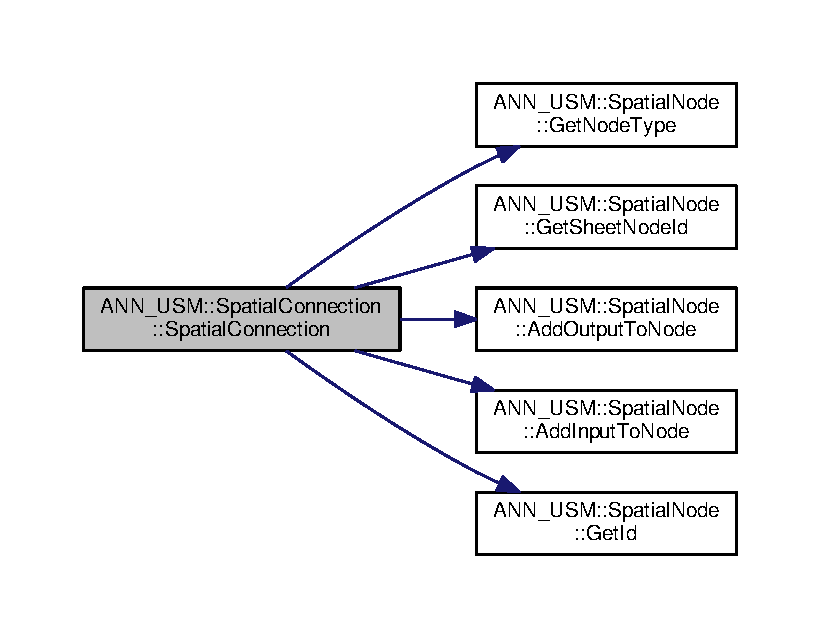
\includegraphics[width=350pt]{class_a_n_n___u_s_m_1_1_spatial_connection_a2043e25434c9f6de7d49f878499b40c9_cgraph}
\end{center}
\end{figure}


\hypertarget{class_a_n_n___u_s_m_1_1_spatial_connection_a9965054cf2e32331a537ed19f79f9c1b}{\index{A\-N\-N\-\_\-\-U\-S\-M\-::\-Spatial\-Connection@{A\-N\-N\-\_\-\-U\-S\-M\-::\-Spatial\-Connection}!$\sim$\-Spatial\-Connection@{$\sim$\-Spatial\-Connection}}
\index{$\sim$\-Spatial\-Connection@{$\sim$\-Spatial\-Connection}!ANN_USM::SpatialConnection@{A\-N\-N\-\_\-\-U\-S\-M\-::\-Spatial\-Connection}}
\subsubsection[{$\sim$\-Spatial\-Connection}]{\setlength{\rightskip}{0pt plus 5cm}Spatial\-Connection\-::$\sim$\-Spatial\-Connection (
\begin{DoxyParamCaption}
{}
\end{DoxyParamCaption}
)}}\label{class_a_n_n___u_s_m_1_1_spatial_connection_a9965054cf2e32331a537ed19f79f9c1b}


Destructor. 



Definition at line 28 of file Spatial\-Connection.\-cpp.



\subsection{Member Function Documentation}
\hypertarget{class_a_n_n___u_s_m_1_1_spatial_connection_a6966fadad1b8fc5c538756bd960f5330}{\index{A\-N\-N\-\_\-\-U\-S\-M\-::\-Spatial\-Connection@{A\-N\-N\-\_\-\-U\-S\-M\-::\-Spatial\-Connection}!Evaluate@{Evaluate}}
\index{Evaluate@{Evaluate}!ANN_USM::SpatialConnection@{A\-N\-N\-\_\-\-U\-S\-M\-::\-Spatial\-Connection}}
\subsubsection[{Evaluate}]{\setlength{\rightskip}{0pt plus 5cm}void Spatial\-Connection\-::\-Evaluate (
\begin{DoxyParamCaption}
{}
\end{DoxyParamCaption}
)}}\label{class_a_n_n___u_s_m_1_1_spatial_connection_a6966fadad1b8fc5c538756bd960f5330}


Evalue the spatial connection output. 



Definition at line 31 of file Spatial\-Connection.\-cpp.

\hypertarget{class_a_n_n___u_s_m_1_1_spatial_connection_a87292c3fa64b90b2e4ab8f5c76960002}{\index{A\-N\-N\-\_\-\-U\-S\-M\-::\-Spatial\-Connection@{A\-N\-N\-\_\-\-U\-S\-M\-::\-Spatial\-Connection}!Get\-Input\-Coordenates@{Get\-Input\-Coordenates}}
\index{Get\-Input\-Coordenates@{Get\-Input\-Coordenates}!ANN_USM::SpatialConnection@{A\-N\-N\-\_\-\-U\-S\-M\-::\-Spatial\-Connection}}
\subsubsection[{Get\-Input\-Coordenates}]{\setlength{\rightskip}{0pt plus 5cm}vector$<$ double $>$ Spatial\-Connection\-::\-Get\-Input\-Coordenates (
\begin{DoxyParamCaption}
{}
\end{DoxyParamCaption}
)}}\label{class_a_n_n___u_s_m_1_1_spatial_connection_a87292c3fa64b90b2e4ab8f5c76960002}


Get the input node cordenates. 

\begin{DoxyReturn}{Returns}
Vector of coordenates 
\end{DoxyReturn}


Definition at line 37 of file Spatial\-Connection.\-cpp.



Here is the call graph for this function\-:
\nopagebreak
\begin{figure}[H]
\begin{center}
\leavevmode
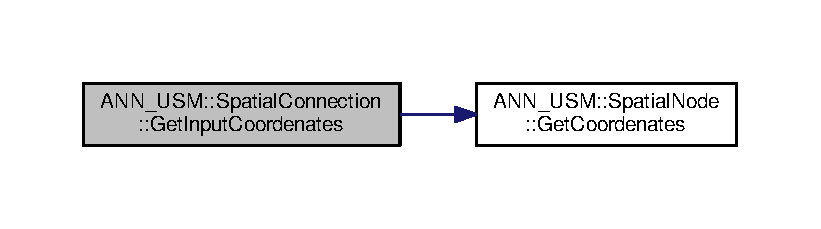
\includegraphics[width=350pt]{class_a_n_n___u_s_m_1_1_spatial_connection_a87292c3fa64b90b2e4ab8f5c76960002_cgraph}
\end{center}
\end{figure}


\hypertarget{class_a_n_n___u_s_m_1_1_spatial_connection_ab8a8bbebac081e28ef8a2a537168cd7b}{\index{A\-N\-N\-\_\-\-U\-S\-M\-::\-Spatial\-Connection@{A\-N\-N\-\_\-\-U\-S\-M\-::\-Spatial\-Connection}!Get\-Output\-Coordenates@{Get\-Output\-Coordenates}}
\index{Get\-Output\-Coordenates@{Get\-Output\-Coordenates}!ANN_USM::SpatialConnection@{A\-N\-N\-\_\-\-U\-S\-M\-::\-Spatial\-Connection}}
\subsubsection[{Get\-Output\-Coordenates}]{\setlength{\rightskip}{0pt plus 5cm}vector$<$ double $>$ Spatial\-Connection\-::\-Get\-Output\-Coordenates (
\begin{DoxyParamCaption}
{}
\end{DoxyParamCaption}
)}}\label{class_a_n_n___u_s_m_1_1_spatial_connection_ab8a8bbebac081e28ef8a2a537168cd7b}


Get the output node coordenates. 

\begin{DoxyReturn}{Returns}
Vector of coordenates 
\end{DoxyReturn}


Definition at line 40 of file Spatial\-Connection.\-cpp.



Here is the call graph for this function\-:
\nopagebreak
\begin{figure}[H]
\begin{center}
\leavevmode
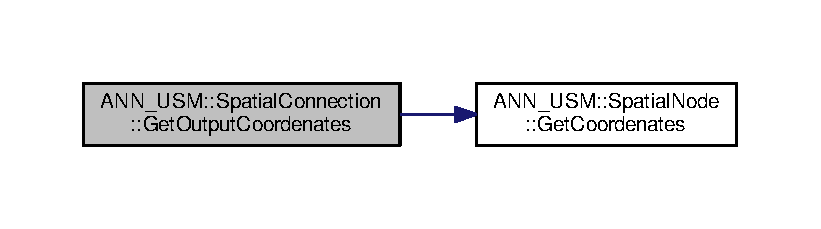
\includegraphics[width=350pt]{class_a_n_n___u_s_m_1_1_spatial_connection_ab8a8bbebac081e28ef8a2a537168cd7b_cgraph}
\end{center}
\end{figure}




The documentation for this class was generated from the following files\-:\begin{DoxyCompactItemize}
\item 
headers/\hyperlink{_spatial_connection_8hpp}{Spatial\-Connection.\-hpp}\item 
src/\hyperlink{_spatial_connection_8cpp}{Spatial\-Connection.\-cpp}\end{DoxyCompactItemize}

\hypertarget{class_a_n_n___u_s_m_1_1_spatial_node}{\section{A\-N\-N\-\_\-\-U\-S\-M\-:\-:Spatial\-Node Class Reference}
\label{class_a_n_n___u_s_m_1_1_spatial_node}\index{A\-N\-N\-\_\-\-U\-S\-M\-::\-Spatial\-Node@{A\-N\-N\-\_\-\-U\-S\-M\-::\-Spatial\-Node}}
}


The class \hyperlink{class_a_n_n___u_s_m_1_1_spatial_node}{Spatial\-Node} is used to create nodes in a \hyperlink{class_a_n_n___u_s_m_1_1_hyper_neat}{Hyper\-Neat} \hyperlink{class_a_n_n___u_s_m_1_1_substrate}{Substrate}.  




{\ttfamily \#include $<$Spatial\-Node.\-hpp$>$}

\subsection*{Public Member Functions}
\begin{DoxyCompactItemize}
\item 
\hyperlink{class_a_n_n___u_s_m_1_1_spatial_node_a850a0daf46db5285b1e8040290b07674}{Spatial\-Node} (int id, int node\-\_\-type, int sheet\-\_\-id, vector$<$ double $>$ coordenates)
\begin{DoxyCompactList}\small\item\em Constructor with parameters. \end{DoxyCompactList}\item 
\hyperlink{class_a_n_n___u_s_m_1_1_spatial_node_ae336eca0b93593037e499d294d0ad1e9}{Spatial\-Node} ()
\begin{DoxyCompactList}\small\item\em Void constructor. \end{DoxyCompactList}\item 
\hyperlink{class_a_n_n___u_s_m_1_1_spatial_node_abc168ab9247fe8de51cae8fa20ed426f}{$\sim$\-Spatial\-Node} ()
\begin{DoxyCompactList}\small\item\em Desstructor. \end{DoxyCompactList}\item 
void \hyperlink{class_a_n_n___u_s_m_1_1_spatial_node_a766657c75494a2b8a63efa490cd69731}{Set\-Input\-To\-Input\-Node} (double $\ast$input)
\begin{DoxyCompactList}\small\item\em Assign input to input type node. \end{DoxyCompactList}\item 
void \hyperlink{class_a_n_n___u_s_m_1_1_spatial_node_af35108c8493e1d07417cca24647472d2}{Set\-Output\-To\-Output\-Node} (double $\ast$output)
\begin{DoxyCompactList}\small\item\em Assign output to output type node. \end{DoxyCompactList}\item 
void \hyperlink{class_a_n_n___u_s_m_1_1_spatial_node_ae994e1f4b678210c67158bec7c43225f}{Add\-Input\-To\-Node} (double $\ast$input)
\begin{DoxyCompactList}\small\item\em Add input to node with spatial connection. \end{DoxyCompactList}\item 
double $\ast$ \hyperlink{class_a_n_n___u_s_m_1_1_spatial_node_a17635297f3f9938e59c914759eff1e38}{Add\-Output\-To\-Node} ()
\begin{DoxyCompactList}\small\item\em Add output to node with spatial connection. \end{DoxyCompactList}\item 
void \hyperlink{class_a_n_n___u_s_m_1_1_spatial_node_a54be8fc283f882507d1b9c857ceea2ba}{Output\-Calcule} ()
\begin{DoxyCompactList}\small\item\em Calcule of node output value. \end{DoxyCompactList}\item 
vector$<$ double $>$ \hyperlink{class_a_n_n___u_s_m_1_1_spatial_node_aad2b17c6937b3517d331292625d63a48}{Get\-Coordenates} ()
\begin{DoxyCompactList}\small\item\em Get coordenates node. \end{DoxyCompactList}\item 
int \hyperlink{class_a_n_n___u_s_m_1_1_spatial_node_ae0a3083058aed45ba3bb44a3f6fd365d}{Get\-Id} ()
\begin{DoxyCompactList}\small\item\em Get node id. \end{DoxyCompactList}\item 
int \hyperlink{class_a_n_n___u_s_m_1_1_spatial_node_a56243b697d163058971480946ba4c7c9}{Get\-Node\-Type} ()
\begin{DoxyCompactList}\small\item\em Get node type. \end{DoxyCompactList}\item 
int \hyperlink{class_a_n_n___u_s_m_1_1_spatial_node_a6bb17ebc6e8e55ddfbc7f3524ab121f8}{Get\-Sheet\-Node\-Id} ()
\begin{DoxyCompactList}\small\item\em Get sheet node id. \end{DoxyCompactList}\item 
double \hyperlink{class_a_n_n___u_s_m_1_1_spatial_node_aa5f3c5395f1412e56f7becd988a8771c}{Get\-Ouput} ()
\begin{DoxyCompactList}\small\item\em Get node output. \end{DoxyCompactList}\item 
void \hyperlink{class_a_n_n___u_s_m_1_1_spatial_node_a5d7507e42443c893ba7e8c2861a0d344}{Clear\-Inputs} ()
\begin{DoxyCompactList}\small\item\em Clear inputs node vector. \end{DoxyCompactList}\end{DoxyCompactItemize}


\subsection{Detailed Description}
The class \hyperlink{class_a_n_n___u_s_m_1_1_spatial_node}{Spatial\-Node} is used to create nodes in a \hyperlink{class_a_n_n___u_s_m_1_1_hyper_neat}{Hyper\-Neat} \hyperlink{class_a_n_n___u_s_m_1_1_substrate}{Substrate}. 

Definition at line 16 of file Spatial\-Node.\-hpp.



\subsection{Constructor \& Destructor Documentation}
\hypertarget{class_a_n_n___u_s_m_1_1_spatial_node_a850a0daf46db5285b1e8040290b07674}{\index{A\-N\-N\-\_\-\-U\-S\-M\-::\-Spatial\-Node@{A\-N\-N\-\_\-\-U\-S\-M\-::\-Spatial\-Node}!Spatial\-Node@{Spatial\-Node}}
\index{Spatial\-Node@{Spatial\-Node}!ANN_USM::SpatialNode@{A\-N\-N\-\_\-\-U\-S\-M\-::\-Spatial\-Node}}
\subsubsection[{Spatial\-Node}]{\setlength{\rightskip}{0pt plus 5cm}Spatial\-Node\-::\-Spatial\-Node (
\begin{DoxyParamCaption}
\item[{int}]{id, }
\item[{int}]{node\-\_\-type, }
\item[{int}]{sheet\-\_\-id, }
\item[{vector$<$ double $>$}]{coordenates}
\end{DoxyParamCaption}
)}}\label{class_a_n_n___u_s_m_1_1_spatial_node_a850a0daf46db5285b1e8040290b07674}


Constructor with parameters. 


\begin{DoxyParams}{Parameters}
{\em id} & Id value \\
\hline
{\em node\-\_\-type} & Node type value \\
\hline
{\em sheet\-\_\-id} & Sheet id value \\
\hline
{\em coordenates} & Coordenate node vector \\
\hline
\end{DoxyParams}


Definition at line 7 of file Spatial\-Node.\-cpp.

\hypertarget{class_a_n_n___u_s_m_1_1_spatial_node_ae336eca0b93593037e499d294d0ad1e9}{\index{A\-N\-N\-\_\-\-U\-S\-M\-::\-Spatial\-Node@{A\-N\-N\-\_\-\-U\-S\-M\-::\-Spatial\-Node}!Spatial\-Node@{Spatial\-Node}}
\index{Spatial\-Node@{Spatial\-Node}!ANN_USM::SpatialNode@{A\-N\-N\-\_\-\-U\-S\-M\-::\-Spatial\-Node}}
\subsubsection[{Spatial\-Node}]{\setlength{\rightskip}{0pt plus 5cm}Spatial\-Node\-::\-Spatial\-Node (
\begin{DoxyParamCaption}
{}
\end{DoxyParamCaption}
)}}\label{class_a_n_n___u_s_m_1_1_spatial_node_ae336eca0b93593037e499d294d0ad1e9}


Void constructor. 



Definition at line 15 of file Spatial\-Node.\-cpp.

\hypertarget{class_a_n_n___u_s_m_1_1_spatial_node_abc168ab9247fe8de51cae8fa20ed426f}{\index{A\-N\-N\-\_\-\-U\-S\-M\-::\-Spatial\-Node@{A\-N\-N\-\_\-\-U\-S\-M\-::\-Spatial\-Node}!$\sim$\-Spatial\-Node@{$\sim$\-Spatial\-Node}}
\index{$\sim$\-Spatial\-Node@{$\sim$\-Spatial\-Node}!ANN_USM::SpatialNode@{A\-N\-N\-\_\-\-U\-S\-M\-::\-Spatial\-Node}}
\subsubsection[{$\sim$\-Spatial\-Node}]{\setlength{\rightskip}{0pt plus 5cm}Spatial\-Node\-::$\sim$\-Spatial\-Node (
\begin{DoxyParamCaption}
{}
\end{DoxyParamCaption}
)}}\label{class_a_n_n___u_s_m_1_1_spatial_node_abc168ab9247fe8de51cae8fa20ed426f}


Desstructor. 



Definition at line 18 of file Spatial\-Node.\-cpp.



\subsection{Member Function Documentation}
\hypertarget{class_a_n_n___u_s_m_1_1_spatial_node_ae994e1f4b678210c67158bec7c43225f}{\index{A\-N\-N\-\_\-\-U\-S\-M\-::\-Spatial\-Node@{A\-N\-N\-\_\-\-U\-S\-M\-::\-Spatial\-Node}!Add\-Input\-To\-Node@{Add\-Input\-To\-Node}}
\index{Add\-Input\-To\-Node@{Add\-Input\-To\-Node}!ANN_USM::SpatialNode@{A\-N\-N\-\_\-\-U\-S\-M\-::\-Spatial\-Node}}
\subsubsection[{Add\-Input\-To\-Node}]{\setlength{\rightskip}{0pt plus 5cm}void Spatial\-Node\-::\-Add\-Input\-To\-Node (
\begin{DoxyParamCaption}
\item[{double $\ast$}]{input}
\end{DoxyParamCaption}
)}}\label{class_a_n_n___u_s_m_1_1_spatial_node_ae994e1f4b678210c67158bec7c43225f}


Add input to node with spatial connection. 


\begin{DoxyParams}{Parameters}
{\em input} & Input pointer \\
\hline
\end{DoxyParams}


Definition at line 36 of file Spatial\-Node.\-cpp.



Here is the caller graph for this function\-:
\nopagebreak
\begin{figure}[H]
\begin{center}
\leavevmode
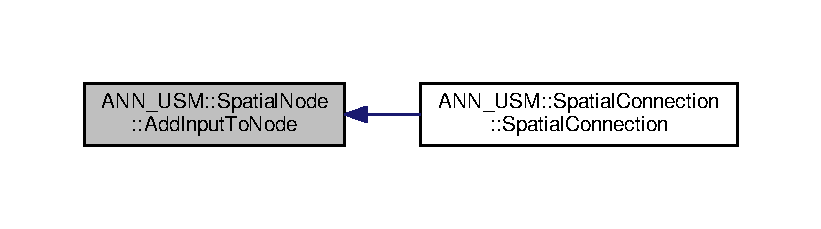
\includegraphics[width=350pt]{class_a_n_n___u_s_m_1_1_spatial_node_ae994e1f4b678210c67158bec7c43225f_icgraph}
\end{center}
\end{figure}


\hypertarget{class_a_n_n___u_s_m_1_1_spatial_node_a17635297f3f9938e59c914759eff1e38}{\index{A\-N\-N\-\_\-\-U\-S\-M\-::\-Spatial\-Node@{A\-N\-N\-\_\-\-U\-S\-M\-::\-Spatial\-Node}!Add\-Output\-To\-Node@{Add\-Output\-To\-Node}}
\index{Add\-Output\-To\-Node@{Add\-Output\-To\-Node}!ANN_USM::SpatialNode@{A\-N\-N\-\_\-\-U\-S\-M\-::\-Spatial\-Node}}
\subsubsection[{Add\-Output\-To\-Node}]{\setlength{\rightskip}{0pt plus 5cm}double $\ast$ Spatial\-Node\-::\-Add\-Output\-To\-Node (
\begin{DoxyParamCaption}
{}
\end{DoxyParamCaption}
)}}\label{class_a_n_n___u_s_m_1_1_spatial_node_a17635297f3f9938e59c914759eff1e38}


Add output to node with spatial connection. 

\begin{DoxyReturn}{Returns}
Output pointer 
\end{DoxyReturn}


Definition at line 41 of file Spatial\-Node.\-cpp.



Here is the caller graph for this function\-:
\nopagebreak
\begin{figure}[H]
\begin{center}
\leavevmode
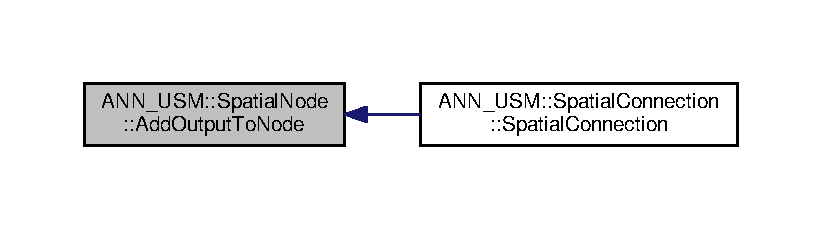
\includegraphics[width=350pt]{class_a_n_n___u_s_m_1_1_spatial_node_a17635297f3f9938e59c914759eff1e38_icgraph}
\end{center}
\end{figure}


\hypertarget{class_a_n_n___u_s_m_1_1_spatial_node_a5d7507e42443c893ba7e8c2861a0d344}{\index{A\-N\-N\-\_\-\-U\-S\-M\-::\-Spatial\-Node@{A\-N\-N\-\_\-\-U\-S\-M\-::\-Spatial\-Node}!Clear\-Inputs@{Clear\-Inputs}}
\index{Clear\-Inputs@{Clear\-Inputs}!ANN_USM::SpatialNode@{A\-N\-N\-\_\-\-U\-S\-M\-::\-Spatial\-Node}}
\subsubsection[{Clear\-Inputs}]{\setlength{\rightskip}{0pt plus 5cm}void Spatial\-Node\-::\-Clear\-Inputs (
\begin{DoxyParamCaption}
{}
\end{DoxyParamCaption}
)}}\label{class_a_n_n___u_s_m_1_1_spatial_node_a5d7507e42443c893ba7e8c2861a0d344}


Clear inputs node vector. 



Definition at line 71 of file Spatial\-Node.\-cpp.

\hypertarget{class_a_n_n___u_s_m_1_1_spatial_node_aad2b17c6937b3517d331292625d63a48}{\index{A\-N\-N\-\_\-\-U\-S\-M\-::\-Spatial\-Node@{A\-N\-N\-\_\-\-U\-S\-M\-::\-Spatial\-Node}!Get\-Coordenates@{Get\-Coordenates}}
\index{Get\-Coordenates@{Get\-Coordenates}!ANN_USM::SpatialNode@{A\-N\-N\-\_\-\-U\-S\-M\-::\-Spatial\-Node}}
\subsubsection[{Get\-Coordenates}]{\setlength{\rightskip}{0pt plus 5cm}vector$<$ double $>$ Spatial\-Node\-::\-Get\-Coordenates (
\begin{DoxyParamCaption}
{}
\end{DoxyParamCaption}
)}}\label{class_a_n_n___u_s_m_1_1_spatial_node_aad2b17c6937b3517d331292625d63a48}


Get coordenates node. 

\begin{DoxyReturn}{Returns}
Coordenate node vector 
\end{DoxyReturn}


Definition at line 56 of file Spatial\-Node.\-cpp.



Here is the caller graph for this function\-:
\nopagebreak
\begin{figure}[H]
\begin{center}
\leavevmode
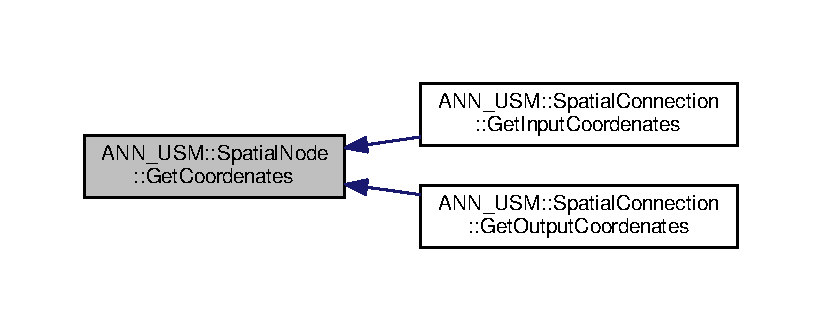
\includegraphics[width=350pt]{class_a_n_n___u_s_m_1_1_spatial_node_aad2b17c6937b3517d331292625d63a48_icgraph}
\end{center}
\end{figure}


\hypertarget{class_a_n_n___u_s_m_1_1_spatial_node_ae0a3083058aed45ba3bb44a3f6fd365d}{\index{A\-N\-N\-\_\-\-U\-S\-M\-::\-Spatial\-Node@{A\-N\-N\-\_\-\-U\-S\-M\-::\-Spatial\-Node}!Get\-Id@{Get\-Id}}
\index{Get\-Id@{Get\-Id}!ANN_USM::SpatialNode@{A\-N\-N\-\_\-\-U\-S\-M\-::\-Spatial\-Node}}
\subsubsection[{Get\-Id}]{\setlength{\rightskip}{0pt plus 5cm}int Spatial\-Node\-::\-Get\-Id (
\begin{DoxyParamCaption}
{}
\end{DoxyParamCaption}
)}}\label{class_a_n_n___u_s_m_1_1_spatial_node_ae0a3083058aed45ba3bb44a3f6fd365d}


Get node id. 

\begin{DoxyReturn}{Returns}
node id value. Input\-: 0, Hidden\-: 1, Output\-: 2 
\end{DoxyReturn}


Definition at line 59 of file Spatial\-Node.\-cpp.



Here is the caller graph for this function\-:
\nopagebreak
\begin{figure}[H]
\begin{center}
\leavevmode
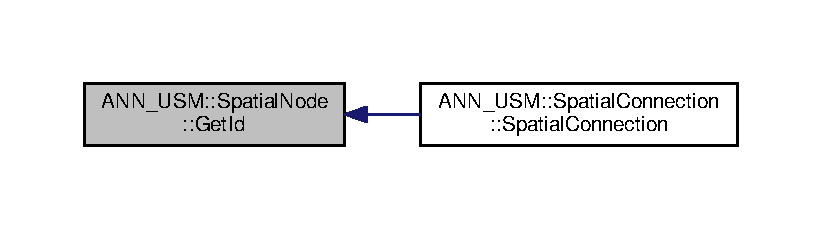
\includegraphics[width=350pt]{class_a_n_n___u_s_m_1_1_spatial_node_ae0a3083058aed45ba3bb44a3f6fd365d_icgraph}
\end{center}
\end{figure}


\hypertarget{class_a_n_n___u_s_m_1_1_spatial_node_a56243b697d163058971480946ba4c7c9}{\index{A\-N\-N\-\_\-\-U\-S\-M\-::\-Spatial\-Node@{A\-N\-N\-\_\-\-U\-S\-M\-::\-Spatial\-Node}!Get\-Node\-Type@{Get\-Node\-Type}}
\index{Get\-Node\-Type@{Get\-Node\-Type}!ANN_USM::SpatialNode@{A\-N\-N\-\_\-\-U\-S\-M\-::\-Spatial\-Node}}
\subsubsection[{Get\-Node\-Type}]{\setlength{\rightskip}{0pt plus 5cm}int Spatial\-Node\-::\-Get\-Node\-Type (
\begin{DoxyParamCaption}
{}
\end{DoxyParamCaption}
)}}\label{class_a_n_n___u_s_m_1_1_spatial_node_a56243b697d163058971480946ba4c7c9}


Get node type. 

\begin{DoxyReturn}{Returns}
node type value 
\end{DoxyReturn}


Definition at line 62 of file Spatial\-Node.\-cpp.



Here is the caller graph for this function\-:
\nopagebreak
\begin{figure}[H]
\begin{center}
\leavevmode
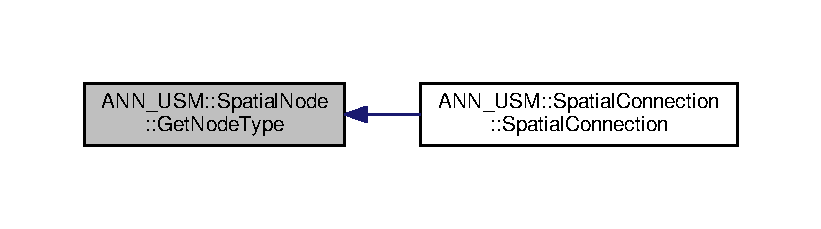
\includegraphics[width=350pt]{class_a_n_n___u_s_m_1_1_spatial_node_a56243b697d163058971480946ba4c7c9_icgraph}
\end{center}
\end{figure}


\hypertarget{class_a_n_n___u_s_m_1_1_spatial_node_aa5f3c5395f1412e56f7becd988a8771c}{\index{A\-N\-N\-\_\-\-U\-S\-M\-::\-Spatial\-Node@{A\-N\-N\-\_\-\-U\-S\-M\-::\-Spatial\-Node}!Get\-Ouput@{Get\-Ouput}}
\index{Get\-Ouput@{Get\-Ouput}!ANN_USM::SpatialNode@{A\-N\-N\-\_\-\-U\-S\-M\-::\-Spatial\-Node}}
\subsubsection[{Get\-Ouput}]{\setlength{\rightskip}{0pt plus 5cm}double Spatial\-Node\-::\-Get\-Ouput (
\begin{DoxyParamCaption}
{}
\end{DoxyParamCaption}
)}}\label{class_a_n_n___u_s_m_1_1_spatial_node_aa5f3c5395f1412e56f7becd988a8771c}


Get node output. 

\begin{DoxyReturn}{Returns}
node output value 
\end{DoxyReturn}


Definition at line 68 of file Spatial\-Node.\-cpp.

\hypertarget{class_a_n_n___u_s_m_1_1_spatial_node_a6bb17ebc6e8e55ddfbc7f3524ab121f8}{\index{A\-N\-N\-\_\-\-U\-S\-M\-::\-Spatial\-Node@{A\-N\-N\-\_\-\-U\-S\-M\-::\-Spatial\-Node}!Get\-Sheet\-Node\-Id@{Get\-Sheet\-Node\-Id}}
\index{Get\-Sheet\-Node\-Id@{Get\-Sheet\-Node\-Id}!ANN_USM::SpatialNode@{A\-N\-N\-\_\-\-U\-S\-M\-::\-Spatial\-Node}}
\subsubsection[{Get\-Sheet\-Node\-Id}]{\setlength{\rightskip}{0pt plus 5cm}int Spatial\-Node\-::\-Get\-Sheet\-Node\-Id (
\begin{DoxyParamCaption}
{}
\end{DoxyParamCaption}
)}}\label{class_a_n_n___u_s_m_1_1_spatial_node_a6bb17ebc6e8e55ddfbc7f3524ab121f8}


Get sheet node id. 

\begin{DoxyReturn}{Returns}
Sheet node id value 
\end{DoxyReturn}


Definition at line 65 of file Spatial\-Node.\-cpp.



Here is the caller graph for this function\-:
\nopagebreak
\begin{figure}[H]
\begin{center}
\leavevmode
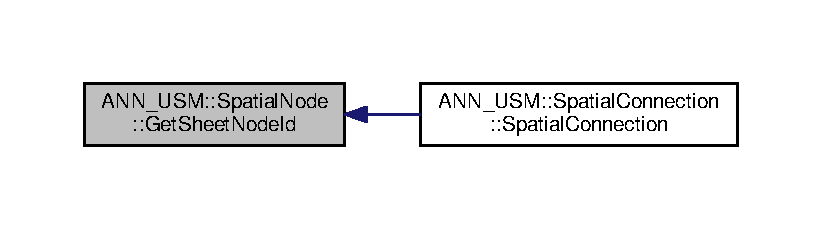
\includegraphics[width=350pt]{class_a_n_n___u_s_m_1_1_spatial_node_a6bb17ebc6e8e55ddfbc7f3524ab121f8_icgraph}
\end{center}
\end{figure}


\hypertarget{class_a_n_n___u_s_m_1_1_spatial_node_a54be8fc283f882507d1b9c857ceea2ba}{\index{A\-N\-N\-\_\-\-U\-S\-M\-::\-Spatial\-Node@{A\-N\-N\-\_\-\-U\-S\-M\-::\-Spatial\-Node}!Output\-Calcule@{Output\-Calcule}}
\index{Output\-Calcule@{Output\-Calcule}!ANN_USM::SpatialNode@{A\-N\-N\-\_\-\-U\-S\-M\-::\-Spatial\-Node}}
\subsubsection[{Output\-Calcule}]{\setlength{\rightskip}{0pt plus 5cm}void Spatial\-Node\-::\-Output\-Calcule (
\begin{DoxyParamCaption}
{}
\end{DoxyParamCaption}
)}}\label{class_a_n_n___u_s_m_1_1_spatial_node_a54be8fc283f882507d1b9c857ceea2ba}


Calcule of node output value. 



Definition at line 44 of file Spatial\-Node.\-cpp.

\hypertarget{class_a_n_n___u_s_m_1_1_spatial_node_a766657c75494a2b8a63efa490cd69731}{\index{A\-N\-N\-\_\-\-U\-S\-M\-::\-Spatial\-Node@{A\-N\-N\-\_\-\-U\-S\-M\-::\-Spatial\-Node}!Set\-Input\-To\-Input\-Node@{Set\-Input\-To\-Input\-Node}}
\index{Set\-Input\-To\-Input\-Node@{Set\-Input\-To\-Input\-Node}!ANN_USM::SpatialNode@{A\-N\-N\-\_\-\-U\-S\-M\-::\-Spatial\-Node}}
\subsubsection[{Set\-Input\-To\-Input\-Node}]{\setlength{\rightskip}{0pt plus 5cm}void Spatial\-Node\-::\-Set\-Input\-To\-Input\-Node (
\begin{DoxyParamCaption}
\item[{double $\ast$}]{input}
\end{DoxyParamCaption}
)}}\label{class_a_n_n___u_s_m_1_1_spatial_node_a766657c75494a2b8a63efa490cd69731}


Assign input to input type node. 


\begin{DoxyParams}{Parameters}
{\em input} & Input pointer \\
\hline
\end{DoxyParams}


Definition at line 22 of file Spatial\-Node.\-cpp.

\hypertarget{class_a_n_n___u_s_m_1_1_spatial_node_af35108c8493e1d07417cca24647472d2}{\index{A\-N\-N\-\_\-\-U\-S\-M\-::\-Spatial\-Node@{A\-N\-N\-\_\-\-U\-S\-M\-::\-Spatial\-Node}!Set\-Output\-To\-Output\-Node@{Set\-Output\-To\-Output\-Node}}
\index{Set\-Output\-To\-Output\-Node@{Set\-Output\-To\-Output\-Node}!ANN_USM::SpatialNode@{A\-N\-N\-\_\-\-U\-S\-M\-::\-Spatial\-Node}}
\subsubsection[{Set\-Output\-To\-Output\-Node}]{\setlength{\rightskip}{0pt plus 5cm}void Spatial\-Node\-::\-Set\-Output\-To\-Output\-Node (
\begin{DoxyParamCaption}
\item[{double $\ast$}]{output}
\end{DoxyParamCaption}
)}}\label{class_a_n_n___u_s_m_1_1_spatial_node_af35108c8493e1d07417cca24647472d2}


Assign output to output type node. 


\begin{DoxyParams}{Parameters}
{\em output} & Output pointer \\
\hline
\end{DoxyParams}


Definition at line 29 of file Spatial\-Node.\-cpp.



The documentation for this class was generated from the following files\-:\begin{DoxyCompactItemize}
\item 
headers/\hyperlink{_spatial_node_8hpp}{Spatial\-Node.\-hpp}\item 
src/\hyperlink{_spatial_node_8cpp}{Spatial\-Node.\-cpp}\end{DoxyCompactItemize}

\hypertarget{class_a_n_n___u_s_m_1_1_substrate}{\section{A\-N\-N\-\_\-\-U\-S\-M\-:\-:Substrate Class Reference}
\label{class_a_n_n___u_s_m_1_1_substrate}\index{A\-N\-N\-\_\-\-U\-S\-M\-::\-Substrate@{A\-N\-N\-\_\-\-U\-S\-M\-::\-Substrate}}
}


The class \hyperlink{class_a_n_n___u_s_m_1_1_substrate}{Substrate} is used to create \hyperlink{class_a_n_n___u_s_m_1_1_hyper_neat}{Hyper\-Neat} \hyperlink{class_a_n_n___u_s_m_1_1_substrate}{Substrate}.  




{\ttfamily \#include $<$Substrate.\-hpp$>$}

\subsection*{Public Member Functions}
\begin{DoxyCompactItemize}
\item 
\hyperlink{class_a_n_n___u_s_m_1_1_substrate_a234055fec868a53cf439fa226b1ae335}{Substrate} (vector$<$ double $\ast$ $>$ inputs, vector$<$ double $\ast$ $>$ outputs)
\begin{DoxyCompactList}\small\item\em Constructor with parameters. \end{DoxyCompactList}\item 
\hyperlink{class_a_n_n___u_s_m_1_1_substrate_a9610e9ffe4266cf149e761ca852a364f}{Substrate} ()
\begin{DoxyCompactList}\small\item\em Void Constructor. \end{DoxyCompactList}\item 
\hyperlink{class_a_n_n___u_s_m_1_1_substrate_a73ad38fceff244a55cfe6ec7ebb46581}{$\sim$\-Substrate} ()
\begin{DoxyCompactList}\small\item\em Destructor. \end{DoxyCompactList}\item 
void \hyperlink{class_a_n_n___u_s_m_1_1_substrate_a5e3ad4577e03d0c4dbb2eef576d0e6a9}{S\-Json\-Deserialize} (char $\ast$substrate\-\_\-info)
\begin{DoxyCompactList}\small\item\em Extract all \hyperlink{class_a_n_n___u_s_m_1_1_substrate}{Substrate} information of char pointer. \end{DoxyCompactList}\item 
void \hyperlink{class_a_n_n___u_s_m_1_1_substrate_a036f4445805ee1d9abf4259e9501118a}{Create\-Nodes} ()
\begin{DoxyCompactList}\small\item\em Inicialize overall nodes based of information extract with S\-Json\-Deserialize function. \end{DoxyCompactList}\item 
int \hyperlink{class_a_n_n___u_s_m_1_1_substrate_a26dee29b17f6d6284969b1697cb69414}{Get\-Layout\-Number} ()
\begin{DoxyCompactList}\small\item\em Get \hyperlink{class_a_n_n___u_s_m_1_1_substrate}{Substrate} layout number. \end{DoxyCompactList}\item 
int \hyperlink{class_a_n_n___u_s_m_1_1_substrate_a01077c74a10333c880c63e4cf2b148c0}{Get\-Coordenate\-Type} (int layout\-\_\-num)
\begin{DoxyCompactList}\small\item\em Get layout coordenate type. \end{DoxyCompactList}\item 
int \hyperlink{class_a_n_n___u_s_m_1_1_substrate_aad34de8fde9ecc3cbb1ebd71548cbc04}{Get\-Layers\-Number} (int layout\-\_\-num)
\begin{DoxyCompactList}\small\item\em Get layout layer number. \end{DoxyCompactList}\item 
int \hyperlink{class_a_n_n___u_s_m_1_1_substrate_af66462bbcfa00eda01f62bf72269860e}{Get\-Layer\-Nodes\-Number} (int layout\-\_\-num, int layer\-\_\-num)
\begin{DoxyCompactList}\small\item\em Get layer node number of specific layout. \end{DoxyCompactList}\item 
\hyperlink{class_a_n_n___u_s_m_1_1_spatial_node}{Spatial\-Node} $\ast$ \hyperlink{class_a_n_n___u_s_m_1_1_substrate_a44672627ec3b103ced54233a29b26486}{Get\-Spatial\-Node} (int layout\-\_\-num, int layer\-\_\-num, int layer\-\_\-node\-\_\-num)
\begin{DoxyCompactList}\small\item\em Get spatial node of specific layout and layer. \end{DoxyCompactList}\item 
void \hyperlink{class_a_n_n___u_s_m_1_1_substrate_a1fc288998e09868f2f8c31e18724106e}{Evaluate\-Spatial\-Node} (int layout\-\_\-num, int layer\-\_\-num)
\begin{DoxyCompactList}\small\item\em Evaluate spatial node outputs of specific layout and layer. \end{DoxyCompactList}\item 
void \hyperlink{class_a_n_n___u_s_m_1_1_substrate_a8c3e61424eede374c5755197a777d354}{Clear\-Spatial\-Node\-Inputs} (int layout\-\_\-num, int layer\-\_\-num)
\begin{DoxyCompactList}\small\item\em Clear input vector of spatial node in specific layout and layer. \end{DoxyCompactList}\item 
double \hyperlink{class_a_n_n___u_s_m_1_1_substrate_a94b7b35d3fff9488ad23f4f8ceb8243b}{Get\-Spatial\-Node\-Output} (int layout\-\_\-num, int layer\-\_\-num, int layer\-\_\-node\-\_\-num)
\begin{DoxyCompactList}\small\item\em Get spatial node output of specific layout and layer. \end{DoxyCompactList}\item 
double \hyperlink{class_a_n_n___u_s_m_1_1_substrate_ab53fac5585cadae2445aec55f84cac43}{Get\-Spatial\-Node\-Id} (int layout\-\_\-num, int layer\-\_\-num, int layer\-\_\-node\-\_\-num)
\begin{DoxyCompactList}\small\item\em Get spatial node id of specific layout and layer. \end{DoxyCompactList}\end{DoxyCompactItemize}


\subsection{Detailed Description}
The class \hyperlink{class_a_n_n___u_s_m_1_1_substrate}{Substrate} is used to create \hyperlink{class_a_n_n___u_s_m_1_1_hyper_neat}{Hyper\-Neat} \hyperlink{class_a_n_n___u_s_m_1_1_substrate}{Substrate}. 

Definition at line 19 of file Substrate.\-hpp.



\subsection{Constructor \& Destructor Documentation}
\hypertarget{class_a_n_n___u_s_m_1_1_substrate_a234055fec868a53cf439fa226b1ae335}{\index{A\-N\-N\-\_\-\-U\-S\-M\-::\-Substrate@{A\-N\-N\-\_\-\-U\-S\-M\-::\-Substrate}!Substrate@{Substrate}}
\index{Substrate@{Substrate}!ANN_USM::Substrate@{A\-N\-N\-\_\-\-U\-S\-M\-::\-Substrate}}
\subsubsection[{Substrate}]{\setlength{\rightskip}{0pt plus 5cm}Substrate\-::\-Substrate (
\begin{DoxyParamCaption}
\item[{vector$<$ double $\ast$ $>$}]{inputs, }
\item[{vector$<$ double $\ast$ $>$}]{outputs}
\end{DoxyParamCaption}
)}}\label{class_a_n_n___u_s_m_1_1_substrate_a234055fec868a53cf439fa226b1ae335}


Constructor with parameters. 


\begin{DoxyParams}{Parameters}
{\em inputs} & Input vector \\
\hline
{\em outputs} & Output vector \\
\hline
\end{DoxyParams}


Definition at line 7 of file Substrate.\-cpp.

\hypertarget{class_a_n_n___u_s_m_1_1_substrate_a9610e9ffe4266cf149e761ca852a364f}{\index{A\-N\-N\-\_\-\-U\-S\-M\-::\-Substrate@{A\-N\-N\-\_\-\-U\-S\-M\-::\-Substrate}!Substrate@{Substrate}}
\index{Substrate@{Substrate}!ANN_USM::Substrate@{A\-N\-N\-\_\-\-U\-S\-M\-::\-Substrate}}
\subsubsection[{Substrate}]{\setlength{\rightskip}{0pt plus 5cm}Substrate\-::\-Substrate (
\begin{DoxyParamCaption}
{}
\end{DoxyParamCaption}
)}}\label{class_a_n_n___u_s_m_1_1_substrate_a9610e9ffe4266cf149e761ca852a364f}


Void Constructor. 



Definition at line 11 of file Substrate.\-cpp.

\hypertarget{class_a_n_n___u_s_m_1_1_substrate_a73ad38fceff244a55cfe6ec7ebb46581}{\index{A\-N\-N\-\_\-\-U\-S\-M\-::\-Substrate@{A\-N\-N\-\_\-\-U\-S\-M\-::\-Substrate}!$\sim$\-Substrate@{$\sim$\-Substrate}}
\index{$\sim$\-Substrate@{$\sim$\-Substrate}!ANN_USM::Substrate@{A\-N\-N\-\_\-\-U\-S\-M\-::\-Substrate}}
\subsubsection[{$\sim$\-Substrate}]{\setlength{\rightskip}{0pt plus 5cm}Substrate\-::$\sim$\-Substrate (
\begin{DoxyParamCaption}
{}
\end{DoxyParamCaption}
)}}\label{class_a_n_n___u_s_m_1_1_substrate_a73ad38fceff244a55cfe6ec7ebb46581}


Destructor. 



Definition at line 14 of file Substrate.\-cpp.



\subsection{Member Function Documentation}
\hypertarget{class_a_n_n___u_s_m_1_1_substrate_a8c3e61424eede374c5755197a777d354}{\index{A\-N\-N\-\_\-\-U\-S\-M\-::\-Substrate@{A\-N\-N\-\_\-\-U\-S\-M\-::\-Substrate}!Clear\-Spatial\-Node\-Inputs@{Clear\-Spatial\-Node\-Inputs}}
\index{Clear\-Spatial\-Node\-Inputs@{Clear\-Spatial\-Node\-Inputs}!ANN_USM::Substrate@{A\-N\-N\-\_\-\-U\-S\-M\-::\-Substrate}}
\subsubsection[{Clear\-Spatial\-Node\-Inputs}]{\setlength{\rightskip}{0pt plus 5cm}void Substrate\-::\-Clear\-Spatial\-Node\-Inputs (
\begin{DoxyParamCaption}
\item[{int}]{layout\-\_\-num, }
\item[{int}]{layer\-\_\-num}
\end{DoxyParamCaption}
)}}\label{class_a_n_n___u_s_m_1_1_substrate_a8c3e61424eede374c5755197a777d354}


Clear input vector of spatial node in specific layout and layer. 


\begin{DoxyParams}{Parameters}
{\em layout\-\_\-num} & Layout number \\
\hline
{\em layer\-\_\-num} & Layer number \\
\hline
\end{DoxyParams}


Definition at line 167 of file Substrate.\-cpp.



Here is the caller graph for this function\-:
\nopagebreak
\begin{figure}[H]
\begin{center}
\leavevmode
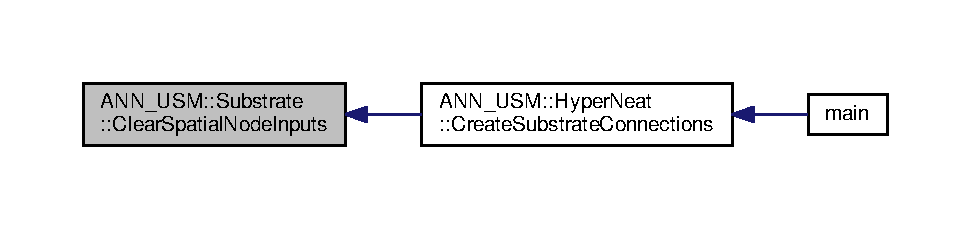
\includegraphics[width=350pt]{class_a_n_n___u_s_m_1_1_substrate_a8c3e61424eede374c5755197a777d354_icgraph}
\end{center}
\end{figure}


\hypertarget{class_a_n_n___u_s_m_1_1_substrate_a036f4445805ee1d9abf4259e9501118a}{\index{A\-N\-N\-\_\-\-U\-S\-M\-::\-Substrate@{A\-N\-N\-\_\-\-U\-S\-M\-::\-Substrate}!Create\-Nodes@{Create\-Nodes}}
\index{Create\-Nodes@{Create\-Nodes}!ANN_USM::Substrate@{A\-N\-N\-\_\-\-U\-S\-M\-::\-Substrate}}
\subsubsection[{Create\-Nodes}]{\setlength{\rightskip}{0pt plus 5cm}void Substrate\-::\-Create\-Nodes (
\begin{DoxyParamCaption}
{}
\end{DoxyParamCaption}
)}}\label{class_a_n_n___u_s_m_1_1_substrate_a036f4445805ee1d9abf4259e9501118a}


Inicialize overall nodes based of information extract with S\-Json\-Deserialize function. 



Definition at line 104 of file Substrate.\-cpp.



Here is the caller graph for this function\-:
\nopagebreak
\begin{figure}[H]
\begin{center}
\leavevmode
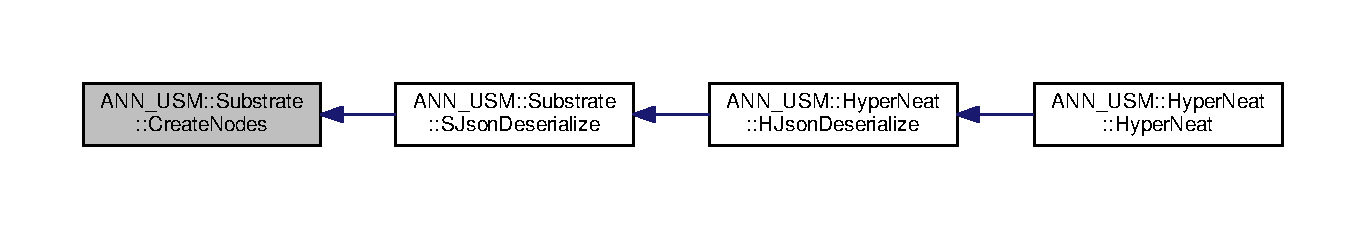
\includegraphics[width=350pt]{class_a_n_n___u_s_m_1_1_substrate_a036f4445805ee1d9abf4259e9501118a_icgraph}
\end{center}
\end{figure}


\hypertarget{class_a_n_n___u_s_m_1_1_substrate_a1fc288998e09868f2f8c31e18724106e}{\index{A\-N\-N\-\_\-\-U\-S\-M\-::\-Substrate@{A\-N\-N\-\_\-\-U\-S\-M\-::\-Substrate}!Evaluate\-Spatial\-Node@{Evaluate\-Spatial\-Node}}
\index{Evaluate\-Spatial\-Node@{Evaluate\-Spatial\-Node}!ANN_USM::Substrate@{A\-N\-N\-\_\-\-U\-S\-M\-::\-Substrate}}
\subsubsection[{Evaluate\-Spatial\-Node}]{\setlength{\rightskip}{0pt plus 5cm}void Substrate\-::\-Evaluate\-Spatial\-Node (
\begin{DoxyParamCaption}
\item[{int}]{layout\-\_\-num, }
\item[{int}]{layer\-\_\-num}
\end{DoxyParamCaption}
)}}\label{class_a_n_n___u_s_m_1_1_substrate_a1fc288998e09868f2f8c31e18724106e}


Evaluate spatial node outputs of specific layout and layer. 


\begin{DoxyParams}{Parameters}
{\em layout\-\_\-num} & Layout number \\
\hline
{\em layer\-\_\-num} & Layer number \\
\hline
\end{DoxyParams}


Definition at line 155 of file Substrate.\-cpp.



Here is the caller graph for this function\-:
\nopagebreak
\begin{figure}[H]
\begin{center}
\leavevmode
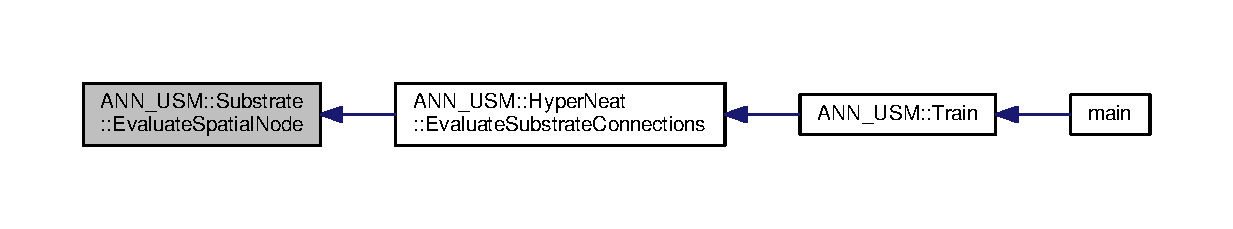
\includegraphics[width=350pt]{class_a_n_n___u_s_m_1_1_substrate_a1fc288998e09868f2f8c31e18724106e_icgraph}
\end{center}
\end{figure}


\hypertarget{class_a_n_n___u_s_m_1_1_substrate_a01077c74a10333c880c63e4cf2b148c0}{\index{A\-N\-N\-\_\-\-U\-S\-M\-::\-Substrate@{A\-N\-N\-\_\-\-U\-S\-M\-::\-Substrate}!Get\-Coordenate\-Type@{Get\-Coordenate\-Type}}
\index{Get\-Coordenate\-Type@{Get\-Coordenate\-Type}!ANN_USM::Substrate@{A\-N\-N\-\_\-\-U\-S\-M\-::\-Substrate}}
\subsubsection[{Get\-Coordenate\-Type}]{\setlength{\rightskip}{0pt plus 5cm}int Substrate\-::\-Get\-Coordenate\-Type (
\begin{DoxyParamCaption}
\item[{int}]{layout\-\_\-num}
\end{DoxyParamCaption}
)}}\label{class_a_n_n___u_s_m_1_1_substrate_a01077c74a10333c880c63e4cf2b148c0}


Get layout coordenate type. 


\begin{DoxyParams}{Parameters}
{\em layout\-\_\-num} & Layout number \\
\hline
\end{DoxyParams}
\begin{DoxyReturn}{Returns}
\hyperlink{class_a_n_n___u_s_m_1_1_substrate}{Substrate} coordenate type 
\end{DoxyReturn}


Definition at line 140 of file Substrate.\-cpp.

\hypertarget{class_a_n_n___u_s_m_1_1_substrate_af66462bbcfa00eda01f62bf72269860e}{\index{A\-N\-N\-\_\-\-U\-S\-M\-::\-Substrate@{A\-N\-N\-\_\-\-U\-S\-M\-::\-Substrate}!Get\-Layer\-Nodes\-Number@{Get\-Layer\-Nodes\-Number}}
\index{Get\-Layer\-Nodes\-Number@{Get\-Layer\-Nodes\-Number}!ANN_USM::Substrate@{A\-N\-N\-\_\-\-U\-S\-M\-::\-Substrate}}
\subsubsection[{Get\-Layer\-Nodes\-Number}]{\setlength{\rightskip}{0pt plus 5cm}int Substrate\-::\-Get\-Layer\-Nodes\-Number (
\begin{DoxyParamCaption}
\item[{int}]{layout\-\_\-num, }
\item[{int}]{layer\-\_\-num}
\end{DoxyParamCaption}
)}}\label{class_a_n_n___u_s_m_1_1_substrate_af66462bbcfa00eda01f62bf72269860e}


Get layer node number of specific layout. 


\begin{DoxyParams}{Parameters}
{\em layout\-\_\-num} & Layout number \\
\hline
{\em layer\-\_\-num} & Layer number \\
\hline
\end{DoxyParams}
\begin{DoxyReturn}{Returns}
Vector of nodes number of each layer in the \hyperlink{class_a_n_n___u_s_m_1_1_substrate}{Substrate} 
\end{DoxyReturn}


Definition at line 146 of file Substrate.\-cpp.



Here is the caller graph for this function\-:
\nopagebreak
\begin{figure}[H]
\begin{center}
\leavevmode
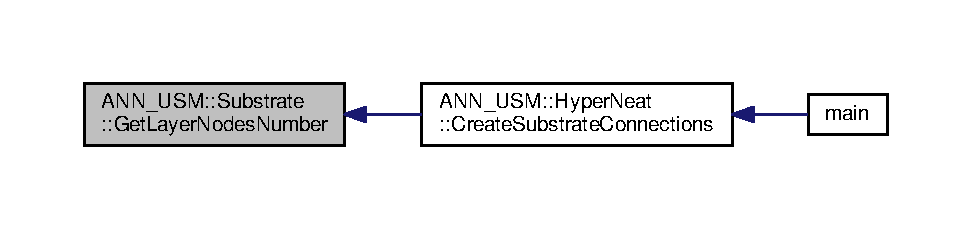
\includegraphics[width=350pt]{class_a_n_n___u_s_m_1_1_substrate_af66462bbcfa00eda01f62bf72269860e_icgraph}
\end{center}
\end{figure}


\hypertarget{class_a_n_n___u_s_m_1_1_substrate_aad34de8fde9ecc3cbb1ebd71548cbc04}{\index{A\-N\-N\-\_\-\-U\-S\-M\-::\-Substrate@{A\-N\-N\-\_\-\-U\-S\-M\-::\-Substrate}!Get\-Layers\-Number@{Get\-Layers\-Number}}
\index{Get\-Layers\-Number@{Get\-Layers\-Number}!ANN_USM::Substrate@{A\-N\-N\-\_\-\-U\-S\-M\-::\-Substrate}}
\subsubsection[{Get\-Layers\-Number}]{\setlength{\rightskip}{0pt plus 5cm}int Substrate\-::\-Get\-Layers\-Number (
\begin{DoxyParamCaption}
\item[{int}]{layout\-\_\-num}
\end{DoxyParamCaption}
)}}\label{class_a_n_n___u_s_m_1_1_substrate_aad34de8fde9ecc3cbb1ebd71548cbc04}


Get layout layer number. 


\begin{DoxyParams}{Parameters}
{\em layout\-\_\-num} & Layout number \\
\hline
\end{DoxyParams}
\begin{DoxyReturn}{Returns}
\hyperlink{class_a_n_n___u_s_m_1_1_substrate}{Substrate} layer number 
\end{DoxyReturn}


Definition at line 143 of file Substrate.\-cpp.



Here is the caller graph for this function\-:
\nopagebreak
\begin{figure}[H]
\begin{center}
\leavevmode
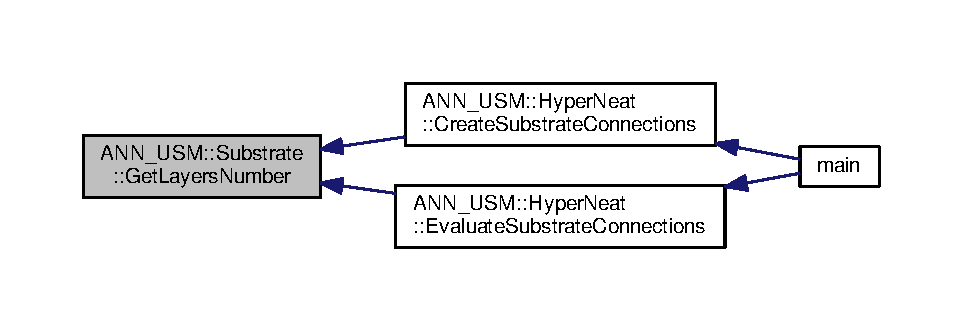
\includegraphics[width=350pt]{class_a_n_n___u_s_m_1_1_substrate_aad34de8fde9ecc3cbb1ebd71548cbc04_icgraph}
\end{center}
\end{figure}


\hypertarget{class_a_n_n___u_s_m_1_1_substrate_a26dee29b17f6d6284969b1697cb69414}{\index{A\-N\-N\-\_\-\-U\-S\-M\-::\-Substrate@{A\-N\-N\-\_\-\-U\-S\-M\-::\-Substrate}!Get\-Layout\-Number@{Get\-Layout\-Number}}
\index{Get\-Layout\-Number@{Get\-Layout\-Number}!ANN_USM::Substrate@{A\-N\-N\-\_\-\-U\-S\-M\-::\-Substrate}}
\subsubsection[{Get\-Layout\-Number}]{\setlength{\rightskip}{0pt plus 5cm}int Substrate\-::\-Get\-Layout\-Number (
\begin{DoxyParamCaption}
{}
\end{DoxyParamCaption}
)}}\label{class_a_n_n___u_s_m_1_1_substrate_a26dee29b17f6d6284969b1697cb69414}


Get \hyperlink{class_a_n_n___u_s_m_1_1_substrate}{Substrate} layout number. 



Definition at line 137 of file Substrate.\-cpp.



Here is the caller graph for this function\-:
\nopagebreak
\begin{figure}[H]
\begin{center}
\leavevmode
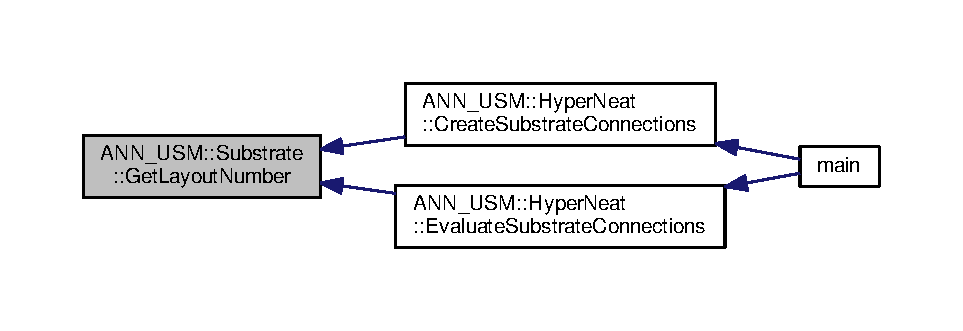
\includegraphics[width=350pt]{class_a_n_n___u_s_m_1_1_substrate_a26dee29b17f6d6284969b1697cb69414_icgraph}
\end{center}
\end{figure}


\hypertarget{class_a_n_n___u_s_m_1_1_substrate_a44672627ec3b103ced54233a29b26486}{\index{A\-N\-N\-\_\-\-U\-S\-M\-::\-Substrate@{A\-N\-N\-\_\-\-U\-S\-M\-::\-Substrate}!Get\-Spatial\-Node@{Get\-Spatial\-Node}}
\index{Get\-Spatial\-Node@{Get\-Spatial\-Node}!ANN_USM::Substrate@{A\-N\-N\-\_\-\-U\-S\-M\-::\-Substrate}}
\subsubsection[{Get\-Spatial\-Node}]{\setlength{\rightskip}{0pt plus 5cm}{\bf Spatial\-Node} $\ast$ Substrate\-::\-Get\-Spatial\-Node (
\begin{DoxyParamCaption}
\item[{int}]{layout\-\_\-num, }
\item[{int}]{layer\-\_\-num, }
\item[{int}]{layer\-\_\-node\-\_\-num}
\end{DoxyParamCaption}
)}}\label{class_a_n_n___u_s_m_1_1_substrate_a44672627ec3b103ced54233a29b26486}


Get spatial node of specific layout and layer. 


\begin{DoxyParams}{Parameters}
{\em layout\-\_\-num} & Layout number \\
\hline
{\em layer\-\_\-num} & Layer number \\
\hline
{\em layer\-\_\-node\-\_\-num} & Layer node number \\
\hline
\end{DoxyParams}
\begin{DoxyReturn}{Returns}
Indicated spatial node pointer 
\end{DoxyReturn}


Definition at line 149 of file Substrate.\-cpp.



Here is the caller graph for this function\-:
\nopagebreak
\begin{figure}[H]
\begin{center}
\leavevmode
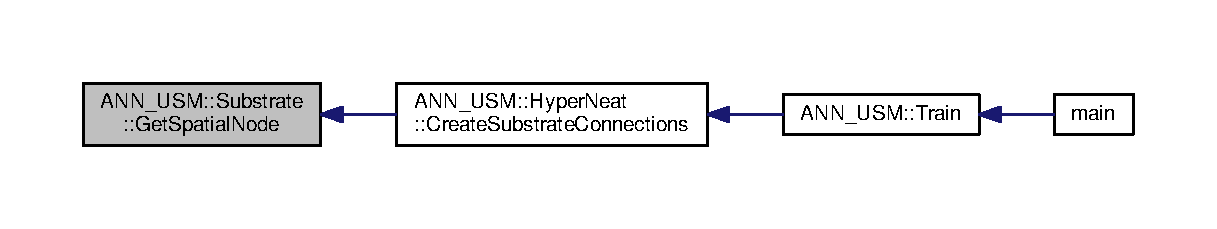
\includegraphics[width=350pt]{class_a_n_n___u_s_m_1_1_substrate_a44672627ec3b103ced54233a29b26486_icgraph}
\end{center}
\end{figure}


\hypertarget{class_a_n_n___u_s_m_1_1_substrate_ab53fac5585cadae2445aec55f84cac43}{\index{A\-N\-N\-\_\-\-U\-S\-M\-::\-Substrate@{A\-N\-N\-\_\-\-U\-S\-M\-::\-Substrate}!Get\-Spatial\-Node\-Id@{Get\-Spatial\-Node\-Id}}
\index{Get\-Spatial\-Node\-Id@{Get\-Spatial\-Node\-Id}!ANN_USM::Substrate@{A\-N\-N\-\_\-\-U\-S\-M\-::\-Substrate}}
\subsubsection[{Get\-Spatial\-Node\-Id}]{\setlength{\rightskip}{0pt plus 5cm}double Substrate\-::\-Get\-Spatial\-Node\-Id (
\begin{DoxyParamCaption}
\item[{int}]{layout\-\_\-num, }
\item[{int}]{layer\-\_\-num, }
\item[{int}]{layer\-\_\-node\-\_\-num}
\end{DoxyParamCaption}
)}}\label{class_a_n_n___u_s_m_1_1_substrate_ab53fac5585cadae2445aec55f84cac43}


Get spatial node id of specific layout and layer. 


\begin{DoxyParams}{Parameters}
{\em layout\-\_\-num} & Layoput number \\
\hline
{\em layer\-\_\-num} & Layer number \\
\hline
{\em layer\-\_\-node\-\_\-num} & Layer node number \\
\hline
\end{DoxyParams}
\begin{DoxyReturn}{Returns}
Id of specific spatial node 
\end{DoxyReturn}


Definition at line 188 of file Substrate.\-cpp.

\hypertarget{class_a_n_n___u_s_m_1_1_substrate_a94b7b35d3fff9488ad23f4f8ceb8243b}{\index{A\-N\-N\-\_\-\-U\-S\-M\-::\-Substrate@{A\-N\-N\-\_\-\-U\-S\-M\-::\-Substrate}!Get\-Spatial\-Node\-Output@{Get\-Spatial\-Node\-Output}}
\index{Get\-Spatial\-Node\-Output@{Get\-Spatial\-Node\-Output}!ANN_USM::Substrate@{A\-N\-N\-\_\-\-U\-S\-M\-::\-Substrate}}
\subsubsection[{Get\-Spatial\-Node\-Output}]{\setlength{\rightskip}{0pt plus 5cm}double Substrate\-::\-Get\-Spatial\-Node\-Output (
\begin{DoxyParamCaption}
\item[{int}]{layout\-\_\-num, }
\item[{int}]{layer\-\_\-num, }
\item[{int}]{layer\-\_\-node\-\_\-num}
\end{DoxyParamCaption}
)}}\label{class_a_n_n___u_s_m_1_1_substrate_a94b7b35d3fff9488ad23f4f8ceb8243b}


Get spatial node output of specific layout and layer. 


\begin{DoxyParams}{Parameters}
{\em layout\-\_\-num} & Layoput number \\
\hline
{\em layer\-\_\-num} & Layer number \\
\hline
{\em layer\-\_\-node\-\_\-num} & Layer node number \\
\hline
\end{DoxyParams}
\begin{DoxyReturn}{Returns}
Output value of specific spatial node 
\end{DoxyReturn}


Definition at line 182 of file Substrate.\-cpp.

\hypertarget{class_a_n_n___u_s_m_1_1_substrate_a5e3ad4577e03d0c4dbb2eef576d0e6a9}{\index{A\-N\-N\-\_\-\-U\-S\-M\-::\-Substrate@{A\-N\-N\-\_\-\-U\-S\-M\-::\-Substrate}!S\-Json\-Deserialize@{S\-Json\-Deserialize}}
\index{S\-Json\-Deserialize@{S\-Json\-Deserialize}!ANN_USM::Substrate@{A\-N\-N\-\_\-\-U\-S\-M\-::\-Substrate}}
\subsubsection[{S\-Json\-Deserialize}]{\setlength{\rightskip}{0pt plus 5cm}void Substrate\-::\-S\-Json\-Deserialize (
\begin{DoxyParamCaption}
\item[{char $\ast$}]{substrate\-\_\-info}
\end{DoxyParamCaption}
)}}\label{class_a_n_n___u_s_m_1_1_substrate_a5e3ad4577e03d0c4dbb2eef576d0e6a9}


Extract all \hyperlink{class_a_n_n___u_s_m_1_1_substrate}{Substrate} information of char pointer. 


\begin{DoxyParams}{Parameters}
{\em substrate\-\_\-info} & char pointer of json string \\
\hline
\end{DoxyParams}


Definition at line 24 of file Substrate.\-cpp.



Here is the call graph for this function\-:
\nopagebreak
\begin{figure}[H]
\begin{center}
\leavevmode
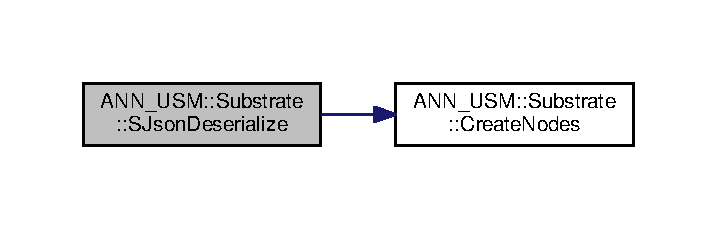
\includegraphics[width=344pt]{class_a_n_n___u_s_m_1_1_substrate_a5e3ad4577e03d0c4dbb2eef576d0e6a9_cgraph}
\end{center}
\end{figure}




Here is the caller graph for this function\-:
\nopagebreak
\begin{figure}[H]
\begin{center}
\leavevmode
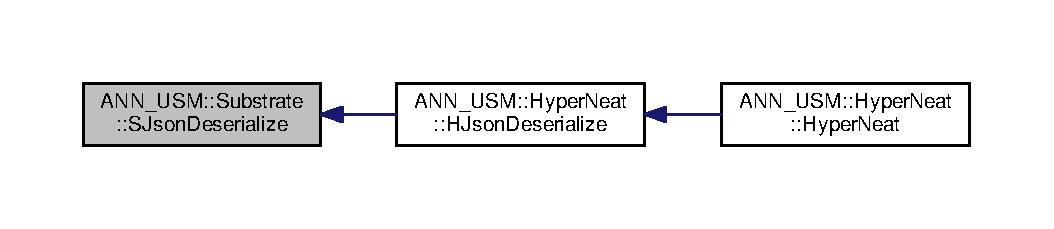
\includegraphics[width=350pt]{class_a_n_n___u_s_m_1_1_substrate_a5e3ad4577e03d0c4dbb2eef576d0e6a9_icgraph}
\end{center}
\end{figure}




The documentation for this class was generated from the following files\-:\begin{DoxyCompactItemize}
\item 
headers/\hyperlink{_substrate_8hpp}{Substrate.\-hpp}\item 
src/\hyperlink{_substrate_8cpp}{Substrate.\-cpp}\end{DoxyCompactItemize}

\chapter{File Documentation}
\hypertarget{_c_p_p_n_inputs_8hpp}{\section{/home/oscar/\-Documents/\-Hyper\-Neat/headers/\-C\-P\-P\-N\-Inputs.hpp File Reference}
\label{_c_p_p_n_inputs_8hpp}\index{/home/oscar/\-Documents/\-Hyper\-Neat/headers/\-C\-P\-P\-N\-Inputs.\-hpp@{/home/oscar/\-Documents/\-Hyper\-Neat/headers/\-C\-P\-P\-N\-Inputs.\-hpp}}
}
{\ttfamily \#include $<$cmath$>$}\\*
{\ttfamily \#include $<$vector$>$}\\*
{\ttfamily \#include $<$cstring$>$}\\*
Include dependency graph for C\-P\-P\-N\-Inputs.\-hpp\-:\nopagebreak
\begin{figure}[H]
\begin{center}
\leavevmode
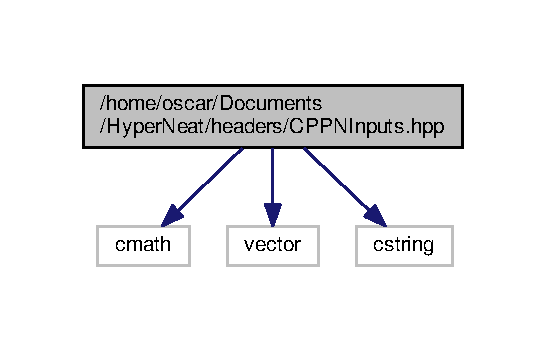
\includegraphics[width=262pt]{_c_p_p_n_inputs_8hpp__incl}
\end{center}
\end{figure}
This graph shows which files directly or indirectly include this file\-:\nopagebreak
\begin{figure}[H]
\begin{center}
\leavevmode
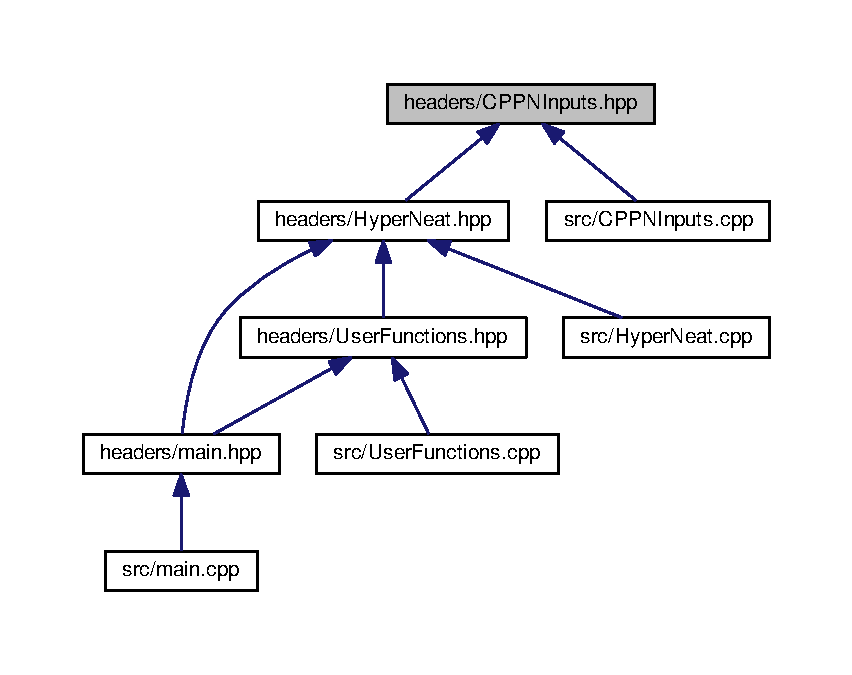
\includegraphics[width=350pt]{_c_p_p_n_inputs_8hpp__dep__incl}
\end{center}
\end{figure}
\subsection*{Classes}
\begin{DoxyCompactItemize}
\item 
class \hyperlink{class_a_n_n___u_s_m_1_1_c_p_p_n_inputs}{A\-N\-N\-\_\-\-U\-S\-M\-::\-C\-P\-P\-N\-Inputs}
\begin{DoxyCompactList}\small\item\em The class \hyperlink{class_a_n_n___u_s_m_1_1_c_p_p_n_inputs}{C\-P\-P\-N\-Inputs} is used to create cppn inputs. \end{DoxyCompactList}\end{DoxyCompactItemize}
\subsection*{Namespaces}
\begin{DoxyCompactItemize}
\item 
\hyperlink{namespace_a_n_n___u_s_m}{A\-N\-N\-\_\-\-U\-S\-M}
\begin{DoxyCompactList}\small\item\em Dedicated to artificial intelligence development in Santa María University. \end{DoxyCompactList}\end{DoxyCompactItemize}

\hypertarget{_hyper_neat_8hpp}{\section{/home/oscar/\-Documents/\-Hyper\-Neat/headers/\-Hyper\-Neat.hpp File Reference}
\label{_hyper_neat_8hpp}\index{/home/oscar/\-Documents/\-Hyper\-Neat/headers/\-Hyper\-Neat.\-hpp@{/home/oscar/\-Documents/\-Hyper\-Neat/headers/\-Hyper\-Neat.\-hpp}}
}
{\ttfamily \#include \char`\"{}Substrate.\-hpp\char`\"{}}\\*
{\ttfamily \#include \char`\"{}Spatial\-Connection.\-hpp\char`\"{}}\\*
{\ttfamily \#include \char`\"{}C\-P\-P\-N\-Inputs.\-hpp\char`\"{}}\\*
{\ttfamily \#include $<$vector$>$}\\*
{\ttfamily \#include $<$string$>$}\\*
{\ttfamily \#include $<$string.\-h$>$}\\*
{\ttfamily \#include $<$iostream$>$}\\*
Include dependency graph for Hyper\-Neat.\-hpp\-:\nopagebreak
\begin{figure}[H]
\begin{center}
\leavevmode
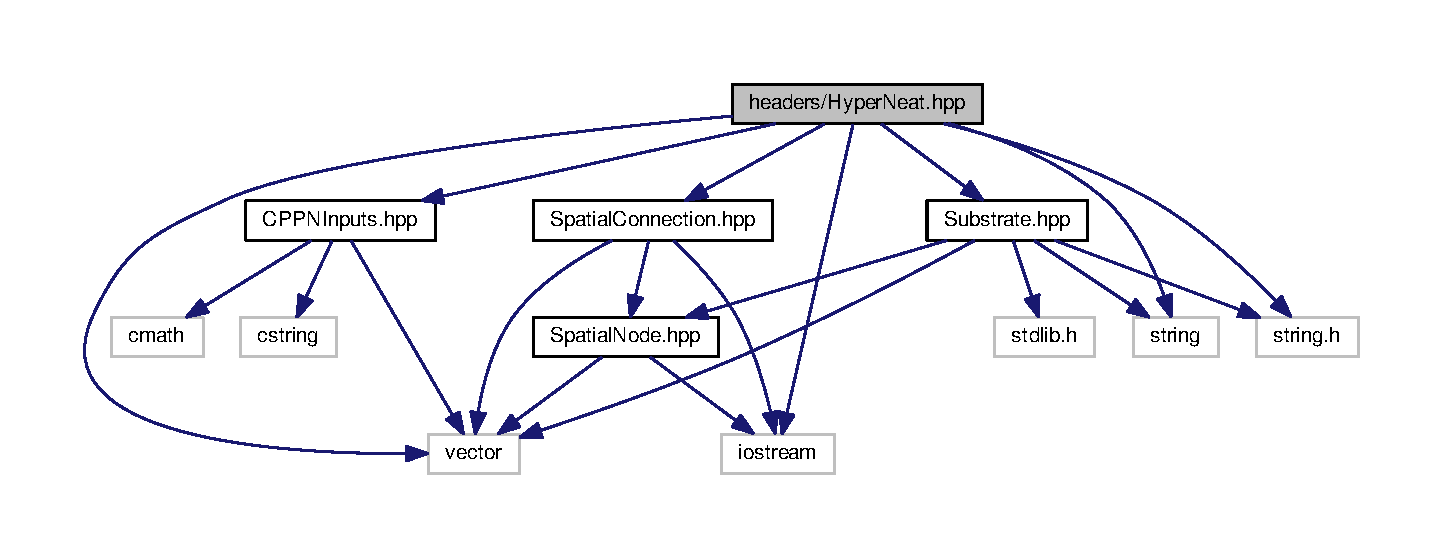
\includegraphics[width=350pt]{_hyper_neat_8hpp__incl}
\end{center}
\end{figure}
This graph shows which files directly or indirectly include this file\-:\nopagebreak
\begin{figure}[H]
\begin{center}
\leavevmode
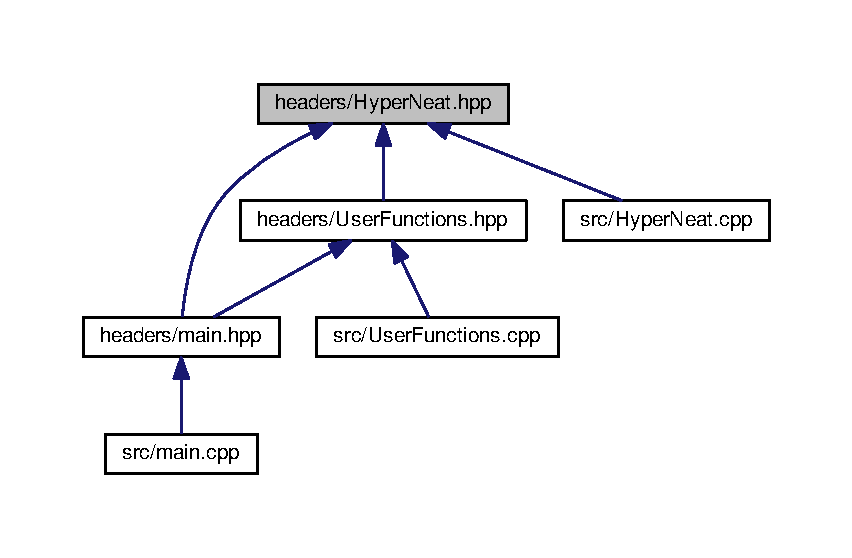
\includegraphics[width=350pt]{_hyper_neat_8hpp__dep__incl}
\end{center}
\end{figure}
\subsection*{Classes}
\begin{DoxyCompactItemize}
\item 
class \hyperlink{class_a_n_n___u_s_m_1_1_hyper_neat}{A\-N\-N\-\_\-\-U\-S\-M\-::\-Hyper\-Neat}
\begin{DoxyCompactList}\small\item\em The class \hyperlink{class_a_n_n___u_s_m_1_1_hyper_neat}{Hyper\-Neat} is used to implement a neuroevolution method called \hyperlink{class_a_n_n___u_s_m_1_1_hyper_neat}{Hyper\-Neat}. \end{DoxyCompactList}\end{DoxyCompactItemize}
\subsection*{Namespaces}
\begin{DoxyCompactItemize}
\item 
\hyperlink{namespace_a_n_n___u_s_m}{A\-N\-N\-\_\-\-U\-S\-M}
\begin{DoxyCompactList}\small\item\em Dedicated to artificial intelligence development in Santa María University. \end{DoxyCompactList}\end{DoxyCompactItemize}

\hypertarget{main_8hpp}{\section{headers/main.hpp File Reference}
\label{main_8hpp}\index{headers/main.\-hpp@{headers/main.\-hpp}}
}
{\ttfamily \#include \char`\"{}Hyper\-Neat.\-hpp\char`\"{}}\\*
{\ttfamily \#include \char`\"{}User\-Functions.\-hpp\char`\"{}}\\*
{\ttfamily \#include $<$vector$>$}\\*
{\ttfamily \#include $<$iostream$>$}\\*
{\ttfamily \#include $<$cstring$>$}\\*
{\ttfamily \#include $<$string$>$}\\*
Include dependency graph for main.\-hpp\-:
\nopagebreak
\begin{figure}[H]
\begin{center}
\leavevmode
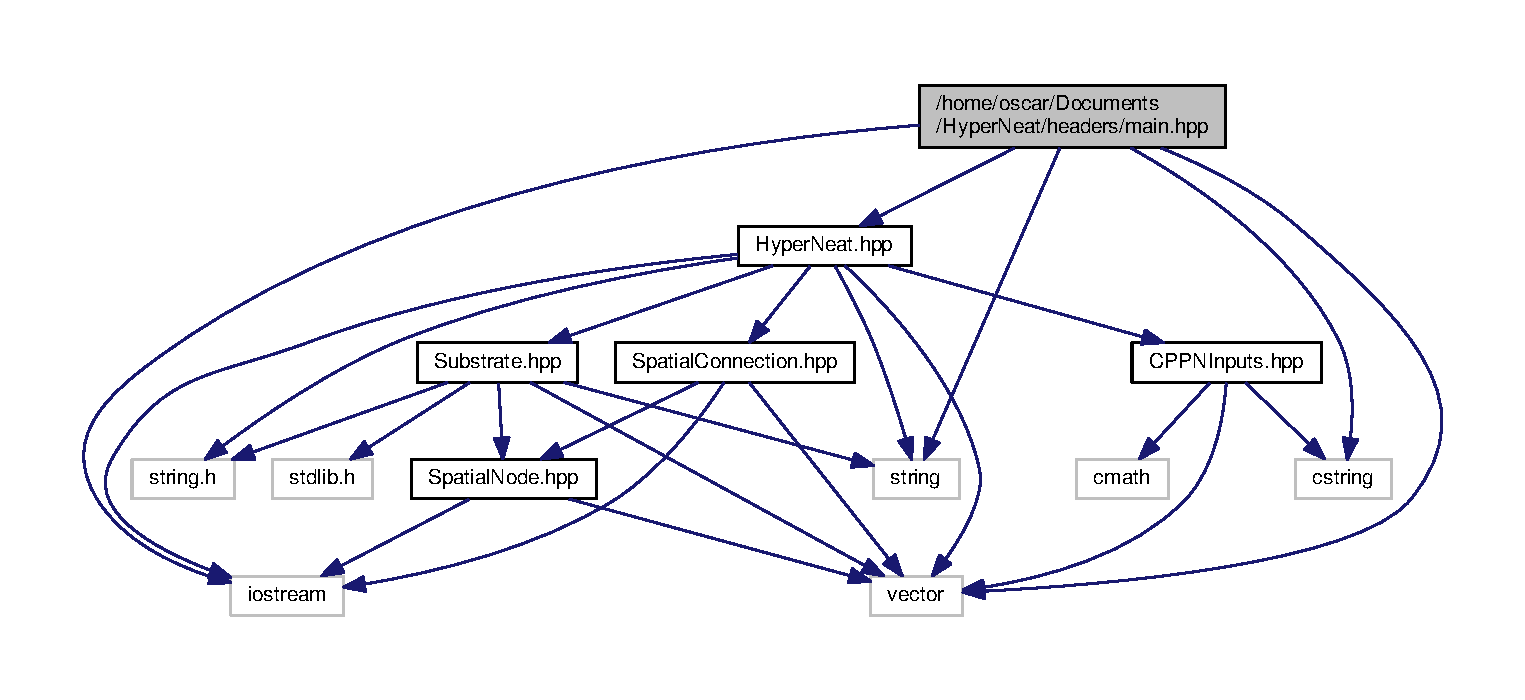
\includegraphics[width=350pt]{main_8hpp__incl}
\end{center}
\end{figure}
This graph shows which files directly or indirectly include this file\-:
\nopagebreak
\begin{figure}[H]
\begin{center}
\leavevmode
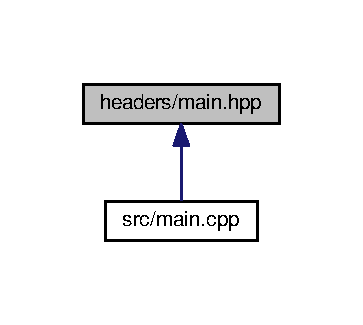
\includegraphics[width=174pt]{main_8hpp__dep__incl}
\end{center}
\end{figure}

\hypertarget{_spatial_connection_8hpp}{\section{headers/\-Spatial\-Connection.hpp File Reference}
\label{_spatial_connection_8hpp}\index{headers/\-Spatial\-Connection.\-hpp@{headers/\-Spatial\-Connection.\-hpp}}
}
{\ttfamily \#include \char`\"{}Spatial\-Node.\-hpp\char`\"{}}\\*
{\ttfamily \#include $<$vector$>$}\\*
{\ttfamily \#include $<$iostream$>$}\\*
Include dependency graph for Spatial\-Connection.\-hpp\-:
\nopagebreak
\begin{figure}[H]
\begin{center}
\leavevmode
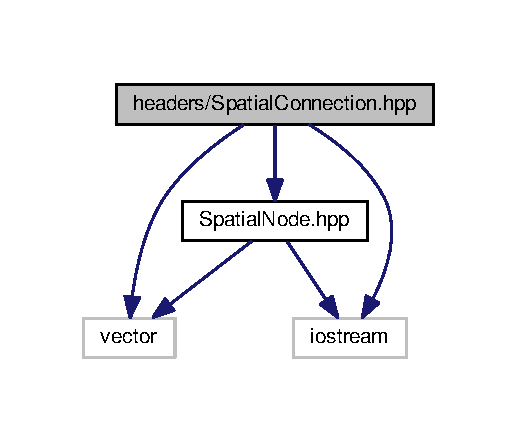
\includegraphics[width=248pt]{_spatial_connection_8hpp__incl}
\end{center}
\end{figure}
This graph shows which files directly or indirectly include this file\-:
\nopagebreak
\begin{figure}[H]
\begin{center}
\leavevmode
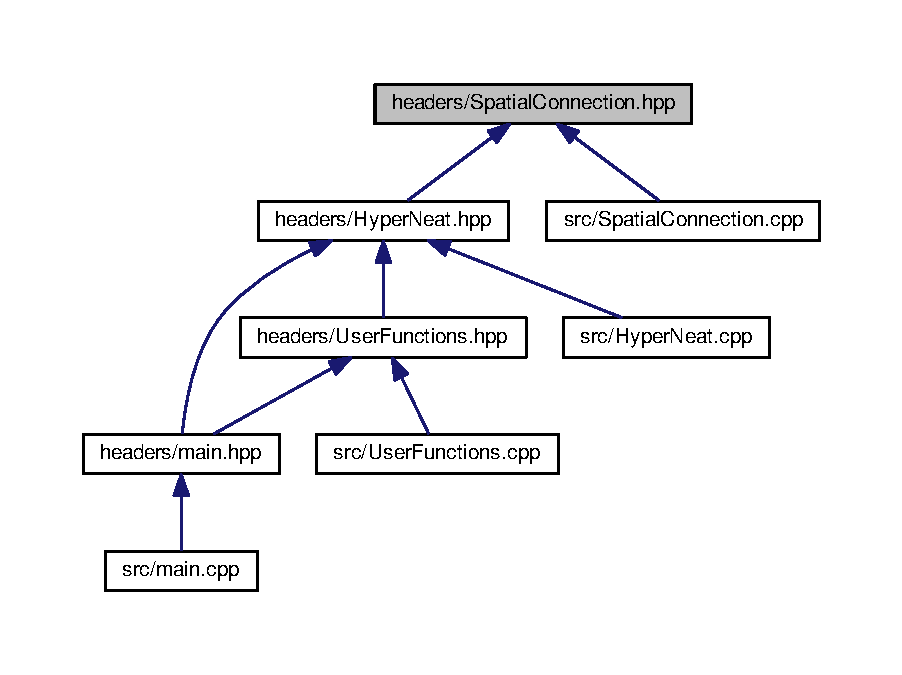
\includegraphics[width=350pt]{_spatial_connection_8hpp__dep__incl}
\end{center}
\end{figure}
\subsection*{Classes}
\begin{DoxyCompactItemize}
\item 
class \hyperlink{class_a_n_n___u_s_m_1_1_spatial_connection}{A\-N\-N\-\_\-\-U\-S\-M\-::\-Spatial\-Connection}
\begin{DoxyCompactList}\small\item\em The class \hyperlink{class_a_n_n___u_s_m_1_1_spatial_connection}{Spatial\-Connection} is used to create connections among overall nodes in a \hyperlink{class_a_n_n___u_s_m_1_1_hyper_neat}{Hyper\-Neat} \hyperlink{class_a_n_n___u_s_m_1_1_substrate}{Substrate}. \end{DoxyCompactList}\end{DoxyCompactItemize}
\subsection*{Namespaces}
\begin{DoxyCompactItemize}
\item 
\hyperlink{namespace_a_n_n___u_s_m}{A\-N\-N\-\_\-\-U\-S\-M}
\begin{DoxyCompactList}\small\item\em Dedicated to artificial intelligence development in Santa María University. \end{DoxyCompactList}\end{DoxyCompactItemize}

\hypertarget{_spatial_node_8hpp}{\section{/home/oscar/\-Documents/\-Hyper\-Neat/headers/\-Spatial\-Node.hpp File Reference}
\label{_spatial_node_8hpp}\index{/home/oscar/\-Documents/\-Hyper\-Neat/headers/\-Spatial\-Node.\-hpp@{/home/oscar/\-Documents/\-Hyper\-Neat/headers/\-Spatial\-Node.\-hpp}}
}
{\ttfamily \#include $<$vector$>$}\\*
{\ttfamily \#include $<$iostream$>$}\\*
Include dependency graph for Spatial\-Node.\-hpp\-:\nopagebreak
\begin{figure}[H]
\begin{center}
\leavevmode
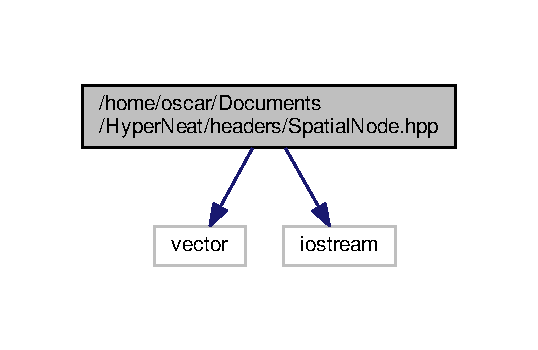
\includegraphics[width=258pt]{_spatial_node_8hpp__incl}
\end{center}
\end{figure}
This graph shows which files directly or indirectly include this file\-:\nopagebreak
\begin{figure}[H]
\begin{center}
\leavevmode
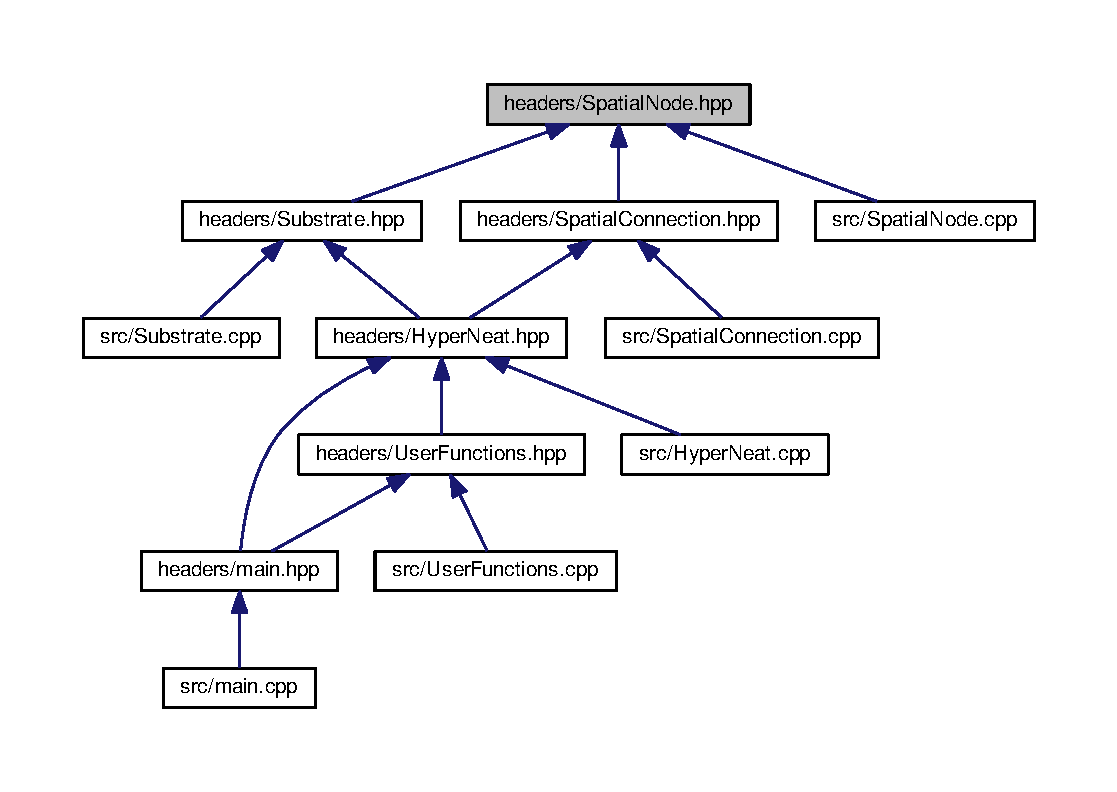
\includegraphics[width=350pt]{_spatial_node_8hpp__dep__incl}
\end{center}
\end{figure}
\subsection*{Classes}
\begin{DoxyCompactItemize}
\item 
class \hyperlink{class_a_n_n___u_s_m_1_1_spatial_node}{A\-N\-N\-\_\-\-U\-S\-M\-::\-Spatial\-Node}
\begin{DoxyCompactList}\small\item\em The class \hyperlink{class_a_n_n___u_s_m_1_1_spatial_node}{Spatial\-Node} is used to create nodes in a \hyperlink{class_a_n_n___u_s_m_1_1_hyper_neat}{Hyper\-Neat} \hyperlink{class_a_n_n___u_s_m_1_1_substrate}{Substrate}. \end{DoxyCompactList}\end{DoxyCompactItemize}
\subsection*{Namespaces}
\begin{DoxyCompactItemize}
\item 
\hyperlink{namespace_a_n_n___u_s_m}{A\-N\-N\-\_\-\-U\-S\-M}
\begin{DoxyCompactList}\small\item\em Dedicated to artificial intelligence development in Santa María University. \end{DoxyCompactList}\end{DoxyCompactItemize}

\hypertarget{_substrate_8hpp}{\section{headers/\-Substrate.hpp File Reference}
\label{_substrate_8hpp}\index{headers/\-Substrate.\-hpp@{headers/\-Substrate.\-hpp}}
}
{\ttfamily \#include $<$vector$>$}\\*
{\ttfamily \#include $<$string$>$}\\*
{\ttfamily \#include $<$string.\-h$>$}\\*
{\ttfamily \#include $<$stdlib.\-h$>$}\\*
{\ttfamily \#include \char`\"{}Spatial\-Node.\-hpp\char`\"{}}\\*
Include dependency graph for Substrate.\-hpp\-:
\nopagebreak
\begin{figure}[H]
\begin{center}
\leavevmode
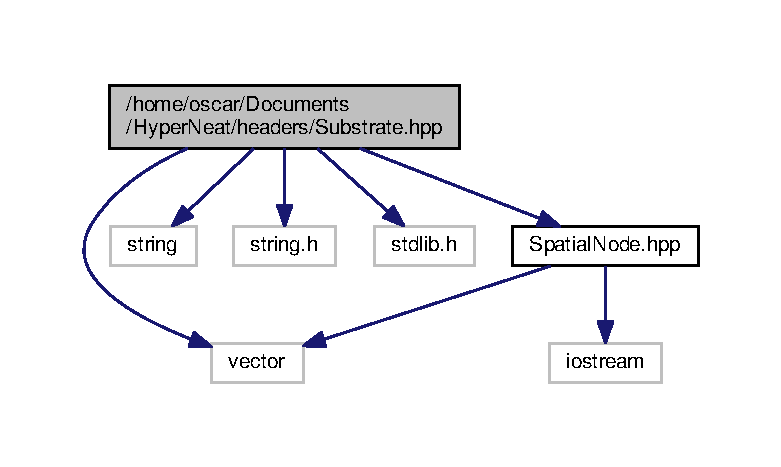
\includegraphics[width=350pt]{_substrate_8hpp__incl}
\end{center}
\end{figure}
This graph shows which files directly or indirectly include this file\-:
\nopagebreak
\begin{figure}[H]
\begin{center}
\leavevmode
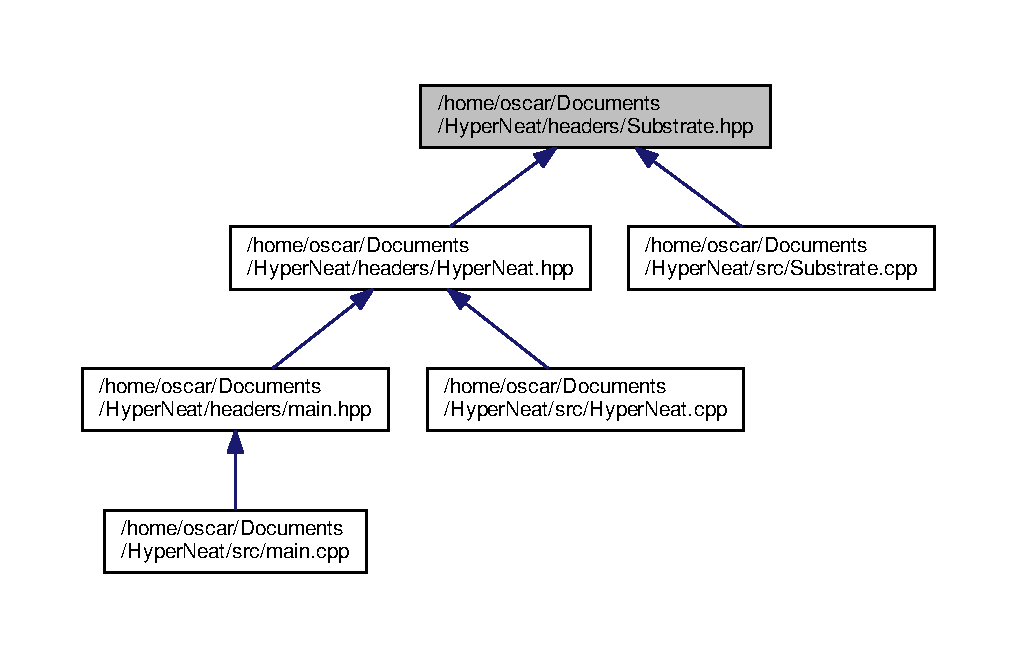
\includegraphics[width=350pt]{_substrate_8hpp__dep__incl}
\end{center}
\end{figure}
\subsection*{Classes}
\begin{DoxyCompactItemize}
\item 
class \hyperlink{class_a_n_n___u_s_m_1_1_substrate}{A\-N\-N\-\_\-\-U\-S\-M\-::\-Substrate}
\begin{DoxyCompactList}\small\item\em The class \hyperlink{class_a_n_n___u_s_m_1_1_substrate}{Substrate} is used to create \hyperlink{class_a_n_n___u_s_m_1_1_hyper_neat}{Hyper\-Neat} \hyperlink{class_a_n_n___u_s_m_1_1_substrate}{Substrate}. \end{DoxyCompactList}\end{DoxyCompactItemize}
\subsection*{Namespaces}
\begin{DoxyCompactItemize}
\item 
\hyperlink{namespace_a_n_n___u_s_m}{A\-N\-N\-\_\-\-U\-S\-M}
\begin{DoxyCompactList}\small\item\em Dedicated to artificial intelligence development in Santa María University. \end{DoxyCompactList}\end{DoxyCompactItemize}

\hypertarget{_c_p_p_n_inputs_8cpp}{\section{src/\-C\-P\-P\-N\-Inputs.cpp File Reference}
\label{_c_p_p_n_inputs_8cpp}\index{src/\-C\-P\-P\-N\-Inputs.\-cpp@{src/\-C\-P\-P\-N\-Inputs.\-cpp}}
}
{\ttfamily \#include \char`\"{}C\-P\-P\-N\-Inputs.\-hpp\char`\"{}}\\*
Include dependency graph for C\-P\-P\-N\-Inputs.\-cpp\-:
\nopagebreak
\begin{figure}[H]
\begin{center}
\leavevmode
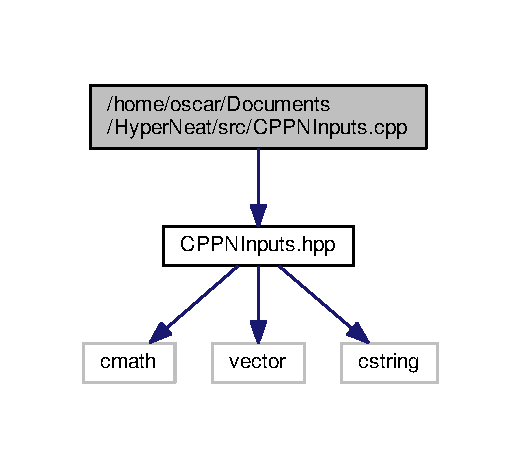
\includegraphics[width=250pt]{_c_p_p_n_inputs_8cpp__incl}
\end{center}
\end{figure}
\subsection*{Macros}
\begin{DoxyCompactItemize}
\item 
\#define \hyperlink{_c_p_p_n_inputs_8cpp_a42b68e6304329ebf6a274dcc7e71bd90}{C\-P\-P\-N\-I\-N\-P\-U\-T\-S\-\_\-\-C\-P\-P}
\end{DoxyCompactItemize}


\subsection{Macro Definition Documentation}
\hypertarget{_c_p_p_n_inputs_8cpp_a42b68e6304329ebf6a274dcc7e71bd90}{\index{C\-P\-P\-N\-Inputs.\-cpp@{C\-P\-P\-N\-Inputs.\-cpp}!C\-P\-P\-N\-I\-N\-P\-U\-T\-S\-\_\-\-C\-P\-P@{C\-P\-P\-N\-I\-N\-P\-U\-T\-S\-\_\-\-C\-P\-P}}
\index{C\-P\-P\-N\-I\-N\-P\-U\-T\-S\-\_\-\-C\-P\-P@{C\-P\-P\-N\-I\-N\-P\-U\-T\-S\-\_\-\-C\-P\-P}!CPPNInputs.cpp@{C\-P\-P\-N\-Inputs.\-cpp}}
\subsubsection[{C\-P\-P\-N\-I\-N\-P\-U\-T\-S\-\_\-\-C\-P\-P}]{\setlength{\rightskip}{0pt plus 5cm}\#define C\-P\-P\-N\-I\-N\-P\-U\-T\-S\-\_\-\-C\-P\-P}}\label{_c_p_p_n_inputs_8cpp_a42b68e6304329ebf6a274dcc7e71bd90}


Definition at line 2 of file C\-P\-P\-N\-Inputs.\-cpp.


\hypertarget{_hyper_neat_8cpp}{\section{src/\-Hyper\-Neat.cpp File Reference}
\label{_hyper_neat_8cpp}\index{src/\-Hyper\-Neat.\-cpp@{src/\-Hyper\-Neat.\-cpp}}
}
{\ttfamily \#include \char`\"{}Hyper\-Neat.\-hpp\char`\"{}}\\*
{\ttfamily \#include $<$unistd.\-h$>$}\\*
Include dependency graph for Hyper\-Neat.\-cpp\-:
\nopagebreak
\begin{figure}[H]
\begin{center}
\leavevmode
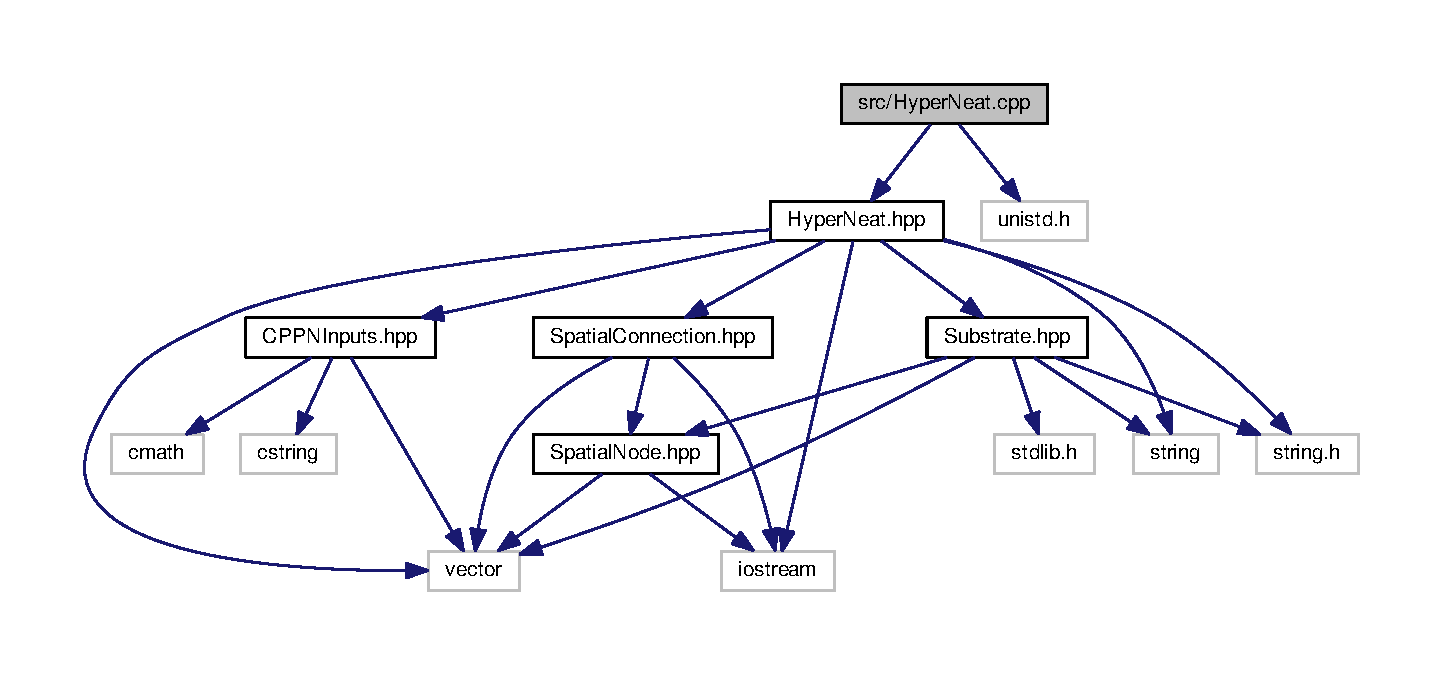
\includegraphics[width=350pt]{_hyper_neat_8cpp__incl}
\end{center}
\end{figure}
\subsection*{Macros}
\begin{DoxyCompactItemize}
\item 
\#define \hyperlink{_hyper_neat_8cpp_aab1e2906aa4e04fb6ebeeafa31d0f607}{H\-Y\-P\-E\-R\-N\-E\-A\-T\-\_\-\-C\-P\-P}
\end{DoxyCompactItemize}


\subsection{Macro Definition Documentation}
\hypertarget{_hyper_neat_8cpp_aab1e2906aa4e04fb6ebeeafa31d0f607}{\index{Hyper\-Neat.\-cpp@{Hyper\-Neat.\-cpp}!H\-Y\-P\-E\-R\-N\-E\-A\-T\-\_\-\-C\-P\-P@{H\-Y\-P\-E\-R\-N\-E\-A\-T\-\_\-\-C\-P\-P}}
\index{H\-Y\-P\-E\-R\-N\-E\-A\-T\-\_\-\-C\-P\-P@{H\-Y\-P\-E\-R\-N\-E\-A\-T\-\_\-\-C\-P\-P}!HyperNeat.cpp@{Hyper\-Neat.\-cpp}}
\subsubsection[{H\-Y\-P\-E\-R\-N\-E\-A\-T\-\_\-\-C\-P\-P}]{\setlength{\rightskip}{0pt plus 5cm}\#define H\-Y\-P\-E\-R\-N\-E\-A\-T\-\_\-\-C\-P\-P}}\label{_hyper_neat_8cpp_aab1e2906aa4e04fb6ebeeafa31d0f607}


Definition at line 2 of file Hyper\-Neat.\-cpp.


\hypertarget{main_8cpp}{\section{src/main.cpp File Reference}
\label{main_8cpp}\index{src/main.\-cpp@{src/main.\-cpp}}
}
{\ttfamily \#include \char`\"{}main.\-hpp\char`\"{}}\\*
{\ttfamily \#include $<$iostream$>$}\\*
Include dependency graph for main.\-cpp\-:
\nopagebreak
\begin{figure}[H]
\begin{center}
\leavevmode
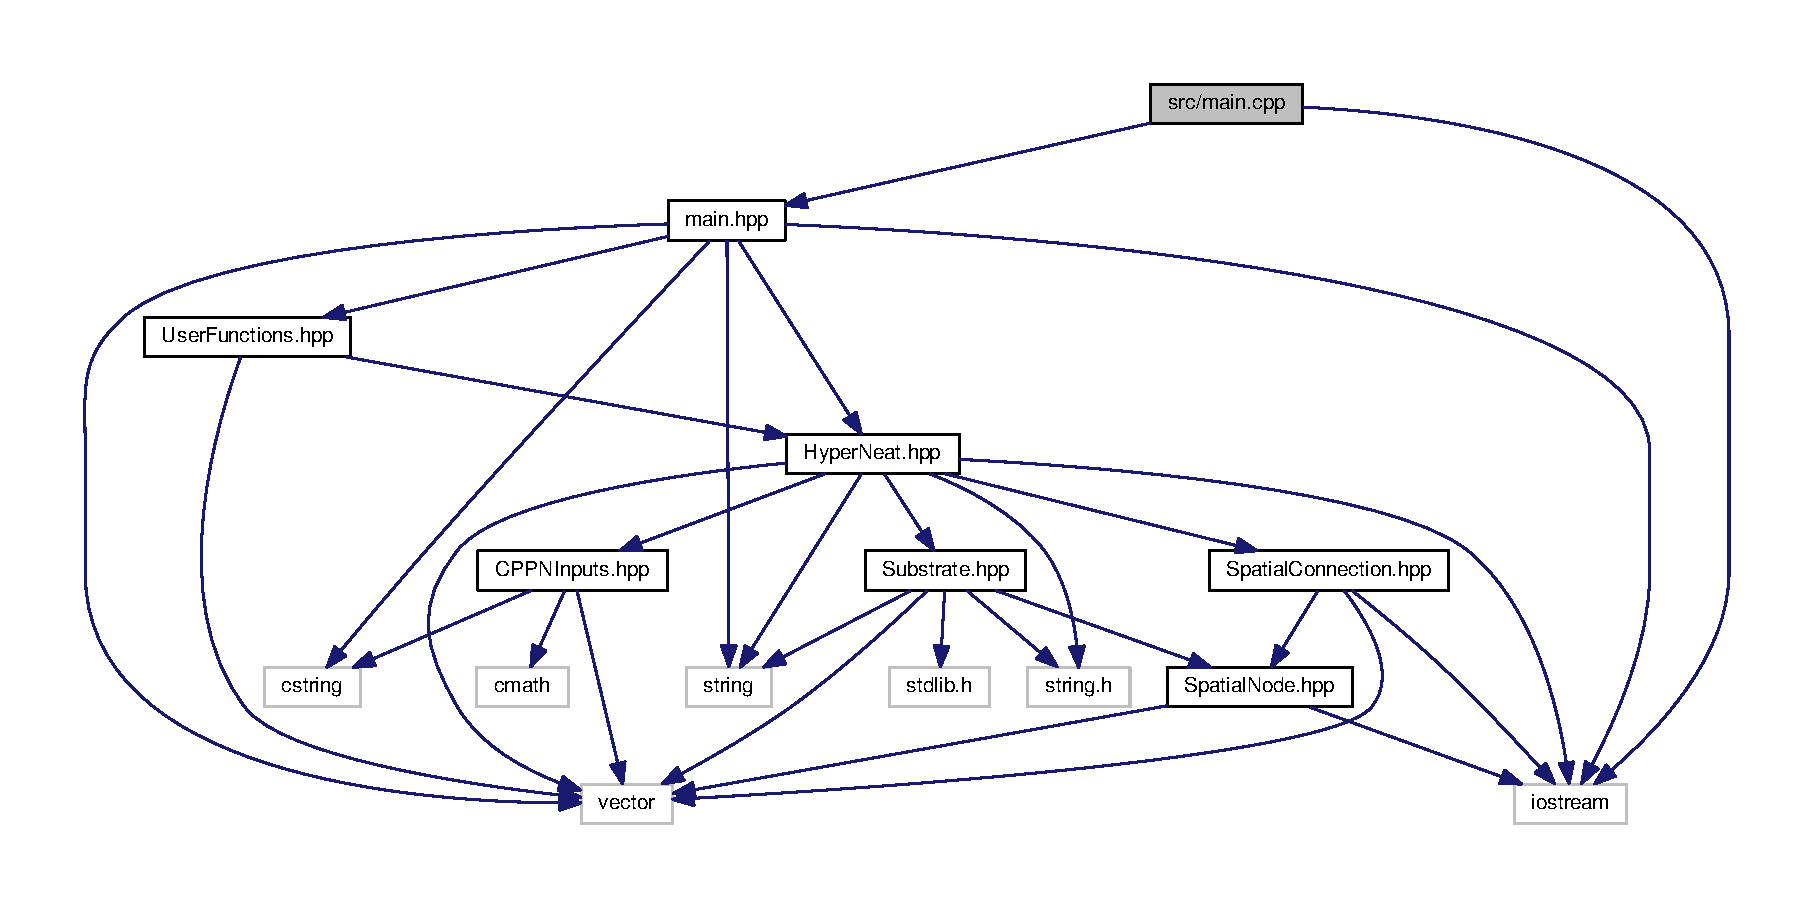
\includegraphics[width=350pt]{main_8cpp__incl}
\end{center}
\end{figure}
\subsection*{Functions}
\begin{DoxyCompactItemize}
\item 
int \hyperlink{main_8cpp_a0ddf1224851353fc92bfbff6f499fa97}{main} (int argc, char $\ast$argv\mbox{[}$\,$\mbox{]})
\end{DoxyCompactItemize}


\subsection{Function Documentation}
\hypertarget{main_8cpp_a0ddf1224851353fc92bfbff6f499fa97}{\index{main.\-cpp@{main.\-cpp}!main@{main}}
\index{main@{main}!main.cpp@{main.\-cpp}}
\subsubsection[{main}]{\setlength{\rightskip}{0pt plus 5cm}int main (
\begin{DoxyParamCaption}
\item[{int}]{argc, }
\item[{char $\ast$}]{argv\mbox{[}$\,$\mbox{]}}
\end{DoxyParamCaption}
)}}\label{main_8cpp_a0ddf1224851353fc92bfbff6f499fa97}


Definition at line 6 of file main.\-cpp.



Here is the call graph for this function\-:
\nopagebreak
\begin{figure}[H]
\begin{center}
\leavevmode
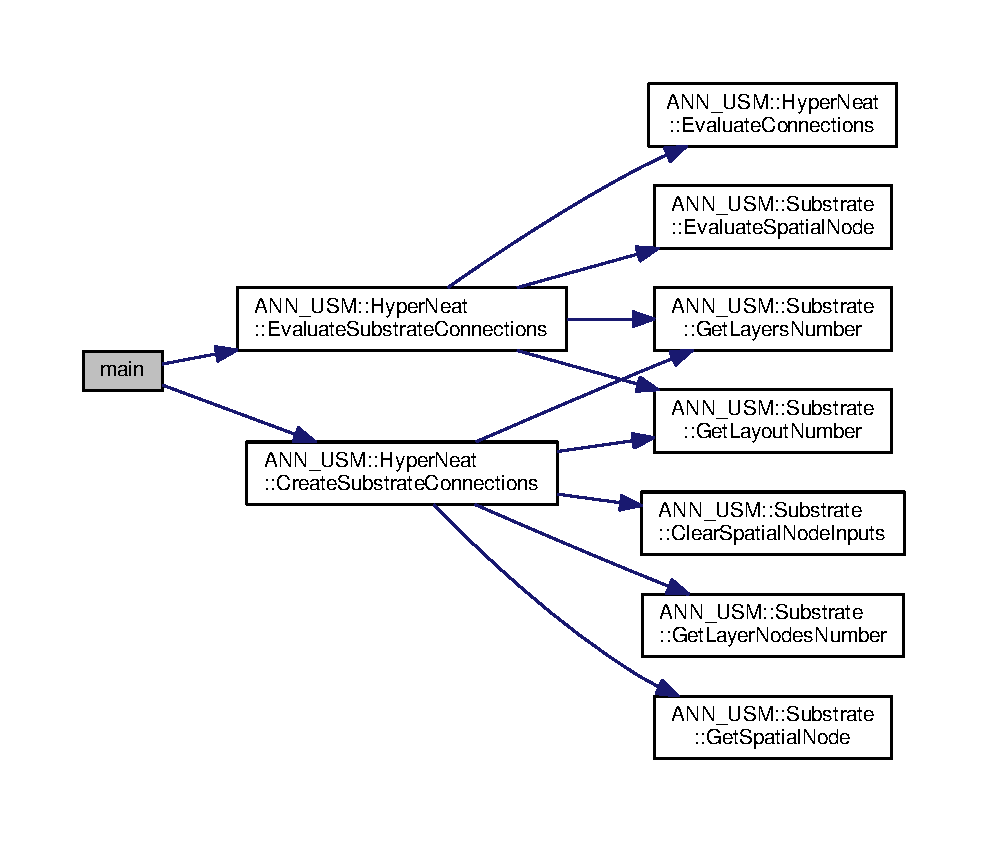
\includegraphics[width=350pt]{main_8cpp_a0ddf1224851353fc92bfbff6f499fa97_cgraph}
\end{center}
\end{figure}



\hypertarget{_spatial_connection_8cpp}{\section{/home/oscar/\-Documents/\-Hyper\-Neat/src/\-Spatial\-Connection.cpp File Reference}
\label{_spatial_connection_8cpp}\index{/home/oscar/\-Documents/\-Hyper\-Neat/src/\-Spatial\-Connection.\-cpp@{/home/oscar/\-Documents/\-Hyper\-Neat/src/\-Spatial\-Connection.\-cpp}}
}
{\ttfamily \#include \char`\"{}Spatial\-Connection.\-hpp\char`\"{}}\\*
Include dependency graph for Spatial\-Connection.\-cpp\-:\nopagebreak
\begin{figure}[H]
\begin{center}
\leavevmode
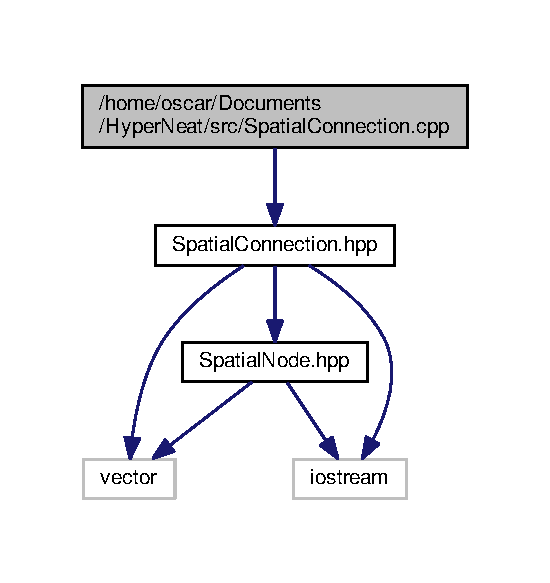
\includegraphics[width=264pt]{_spatial_connection_8cpp__incl}
\end{center}
\end{figure}
\subsection*{Macros}
\begin{DoxyCompactItemize}
\item 
\#define \hyperlink{_spatial_connection_8cpp_a45360bb849fd434d9636afc46dfde818}{S\-P\-A\-T\-I\-A\-L\-C\-O\-N\-N\-E\-C\-T\-I\-O\-N\-\_\-\-C\-P\-P}
\end{DoxyCompactItemize}


\subsection{Macro Definition Documentation}
\hypertarget{_spatial_connection_8cpp_a45360bb849fd434d9636afc46dfde818}{\index{Spatial\-Connection.\-cpp@{Spatial\-Connection.\-cpp}!S\-P\-A\-T\-I\-A\-L\-C\-O\-N\-N\-E\-C\-T\-I\-O\-N\-\_\-\-C\-P\-P@{S\-P\-A\-T\-I\-A\-L\-C\-O\-N\-N\-E\-C\-T\-I\-O\-N\-\_\-\-C\-P\-P}}
\index{S\-P\-A\-T\-I\-A\-L\-C\-O\-N\-N\-E\-C\-T\-I\-O\-N\-\_\-\-C\-P\-P@{S\-P\-A\-T\-I\-A\-L\-C\-O\-N\-N\-E\-C\-T\-I\-O\-N\-\_\-\-C\-P\-P}!SpatialConnection.cpp@{Spatial\-Connection.\-cpp}}
\subsubsection[{S\-P\-A\-T\-I\-A\-L\-C\-O\-N\-N\-E\-C\-T\-I\-O\-N\-\_\-\-C\-P\-P}]{\setlength{\rightskip}{0pt plus 5cm}\#define S\-P\-A\-T\-I\-A\-L\-C\-O\-N\-N\-E\-C\-T\-I\-O\-N\-\_\-\-C\-P\-P}}\label{_spatial_connection_8cpp_a45360bb849fd434d9636afc46dfde818}


Definition at line 2 of file Spatial\-Connection.\-cpp.


\hypertarget{_spatial_node_8cpp}{\section{src/\-Spatial\-Node.cpp File Reference}
\label{_spatial_node_8cpp}\index{src/\-Spatial\-Node.\-cpp@{src/\-Spatial\-Node.\-cpp}}
}
{\ttfamily \#include \char`\"{}Spatial\-Node.\-hpp\char`\"{}}\\*
Include dependency graph for Spatial\-Node.\-cpp\-:
\nopagebreak
\begin{figure}[H]
\begin{center}
\leavevmode
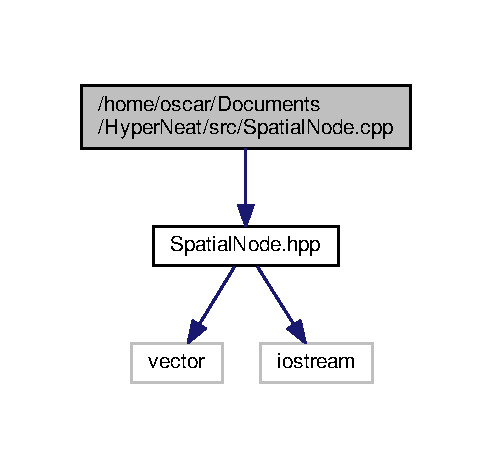
\includegraphics[width=196pt]{_spatial_node_8cpp__incl}
\end{center}
\end{figure}
\subsection*{Macros}
\begin{DoxyCompactItemize}
\item 
\#define \hyperlink{_spatial_node_8cpp_ac0690252610e5127797af312ada1a9fa}{S\-P\-A\-T\-I\-A\-L\-N\-O\-D\-E\-\_\-\-C\-P\-P}
\end{DoxyCompactItemize}


\subsection{Macro Definition Documentation}
\hypertarget{_spatial_node_8cpp_ac0690252610e5127797af312ada1a9fa}{\index{Spatial\-Node.\-cpp@{Spatial\-Node.\-cpp}!S\-P\-A\-T\-I\-A\-L\-N\-O\-D\-E\-\_\-\-C\-P\-P@{S\-P\-A\-T\-I\-A\-L\-N\-O\-D\-E\-\_\-\-C\-P\-P}}
\index{S\-P\-A\-T\-I\-A\-L\-N\-O\-D\-E\-\_\-\-C\-P\-P@{S\-P\-A\-T\-I\-A\-L\-N\-O\-D\-E\-\_\-\-C\-P\-P}!SpatialNode.cpp@{Spatial\-Node.\-cpp}}
\subsubsection[{S\-P\-A\-T\-I\-A\-L\-N\-O\-D\-E\-\_\-\-C\-P\-P}]{\setlength{\rightskip}{0pt plus 5cm}\#define S\-P\-A\-T\-I\-A\-L\-N\-O\-D\-E\-\_\-\-C\-P\-P}}\label{_spatial_node_8cpp_ac0690252610e5127797af312ada1a9fa}


Definition at line 2 of file Spatial\-Node.\-cpp.


\hypertarget{_substrate_8cpp}{\section{src/\-Substrate.cpp File Reference}
\label{_substrate_8cpp}\index{src/\-Substrate.\-cpp@{src/\-Substrate.\-cpp}}
}
{\ttfamily \#include \char`\"{}Substrate.\-hpp\char`\"{}}\\*
Include dependency graph for Substrate.\-cpp\-:
\nopagebreak
\begin{figure}[H]
\begin{center}
\leavevmode
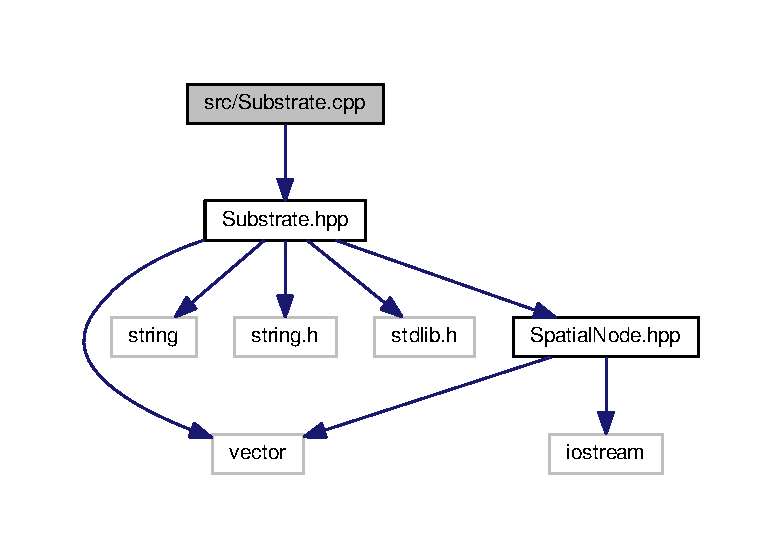
\includegraphics[width=350pt]{_substrate_8cpp__incl}
\end{center}
\end{figure}
\subsection*{Macros}
\begin{DoxyCompactItemize}
\item 
\#define \hyperlink{_substrate_8cpp_a4bb833ed3dda3775106b3c246837ce1e}{S\-U\-B\-S\-T\-R\-A\-T\-E\-\_\-\-C\-P\-P}
\end{DoxyCompactItemize}


\subsection{Macro Definition Documentation}
\hypertarget{_substrate_8cpp_a4bb833ed3dda3775106b3c246837ce1e}{\index{Substrate.\-cpp@{Substrate.\-cpp}!S\-U\-B\-S\-T\-R\-A\-T\-E\-\_\-\-C\-P\-P@{S\-U\-B\-S\-T\-R\-A\-T\-E\-\_\-\-C\-P\-P}}
\index{S\-U\-B\-S\-T\-R\-A\-T\-E\-\_\-\-C\-P\-P@{S\-U\-B\-S\-T\-R\-A\-T\-E\-\_\-\-C\-P\-P}!Substrate.cpp@{Substrate.\-cpp}}
\subsubsection[{S\-U\-B\-S\-T\-R\-A\-T\-E\-\_\-\-C\-P\-P}]{\setlength{\rightskip}{0pt plus 5cm}\#define S\-U\-B\-S\-T\-R\-A\-T\-E\-\_\-\-C\-P\-P}}\label{_substrate_8cpp_a4bb833ed3dda3775106b3c246837ce1e}


Definition at line 2 of file Substrate.\-cpp.


%--- End generated contents ---

% Index
\newpage
\phantomsection
\addcontentsline{toc}{chapter}{Index}
\printindex

\end{document}
